\documentclass[parskip=half, final]{scrreprt}


% General Packages
\usepackage[ngerman]{babel}
\usepackage[xetex]{graphicx}
\usepackage{enumitem}
\usepackage{hyperref}


% Font
\usepackage{fontspec,xunicode}
\setmainfont{Cardo}
\setsansfont{Avenir Next}
\setmonofont[Scale=MatchLowercase]{Menlo} % MatchLowercase is pretty cool


% PDF Meta Info
\makeatletter
\AtBeginDocument{
  \hypersetup{
    pdftitle = {\@title{} \@subtitle},
    pdfauthor = {\@author}
  }
}
\makeatother


% Titlepage
\renewcommand{\maketitle}{
    \begin{titlepage}

\begin{center}

\makeatletter

% Uni
\textsc{
{\LARGE Universität Heidelberg}\\[0.4cm]
{\Large \semester}
}\\[6cm]

% Title
%\newcommand{\HRule}{\rule{\linewidth}{0mm}}
{\Huge \bfseries \@title}\\[1cm]
\textsc{\LARGE \@subtitle}



\vfill


% Author
\textsc{\Large \@author\\[1.5cm]}

% Info
\begin{minipage}{\textwidth}
\begin{flushleft} \large
{\large
Aktualisiert am \today\\
Kursdetails und begleitende Materialien auf der Vorlesungsseite:\\
\emph{http://ios-dev-kurs.github.io}
}
\end{flushleft}
\end{minipage}


\makeatother

\end{center}

\end{titlepage}

}


% Page Layout
%\pagestyle{headings}
\usepackage[textheight=640pt]{geometry}
\usepackage{fancyhdr}
\pagestyle{fancy}
\AtBeginDocument{
\fancyhf{}
\lhead{\textit{Nils Fischer, Universität Heidelberg, \shortsemester}}
\rhead{\textit{\shortdoctype{} \nouppercase{\leftmark}}}
\renewcommand{\headrulewidth}{0.2pt}
\cfoot{\thepage}
}


% Headings
\usepackage[bf]{titlesec}
%\titleformat{\chapter}[display]{\large\bfseries}{\chaptertitlename\ \thechapter}{5pt}{\large}% NEW
%\titlespacing*{\chapter}{0pt}{30pt}{20pt}% NEW


% Menukeys
\usepackage{menukeys}


% Style

\newcommand\strong\textbf

\usepackage{color,xcolor}
\definecolor{string}{RGB}{196,26,22}
\newcommand\str[1]{\textcolor{string}{\texttt{"#1"}}}

\newcommand\filename[1]{\str{#1}}
\newenvironment{filecontent}[1]{\textbf{#1}}{}


% References
\newcommand{\linkref}[1]{[\footnote{\url{#1}}]}
\newcommand{\abbref}[1]{\emph{(\hyperref[#1]{s. S. \pageref{#1}, Abb. \ref{#1}})}}
\newcommand{\secref}[1]{\emph{(\hyperref[#1]{s. S. \pageref{#1}, Abschnitt \ref{#1}})}}
\newcommand{\excref}[1]{\emph{(\hyperref[#1]{s. S. \pageref{#1}, Übungsaufgabe \ref{#1}})}}
\newcommand{\skriptref}[1]{\emph{Relevante Kapitel im Skript: #1}}


% Images
\newcommand{\includegraphicsc}[4][\textwidth]{{\begin{figure}[ht]\centering\includegraphics[width=#1]{#2}\caption{#4}\label{#3}\end{figure}}}
\newcommand{\screenshotwidth}{.8\textwidth}
\newcommand{\iphonewidth}{.4\textwidth}


% Margin Images
\usepackage{marginnote}
\newcommand{\mvcindicatorview}{\reversemarginpar\marginnote{\centering
    
\includegraphics[width=1cm]{img/mvc_view}\\
    \textbf{\small View}
}}
\newcommand{\mvcindicatorcontroller}{\reversemarginpar\marginnote{\centering
    
\includegraphics[width=1cm]{img/mvc_controller}\\
    \textbf{\small Controller}
}}


% Lecture structure
\newenvironment{lecture}{}{\pagebreak}


% Exercise Style
\newcounter{exc}
\newenvironment{exc}{\subsubsection{Übungsaufgaben}\begin{enumerate}\setcounter{enumi}{\theexc}}{\setcounter{exc}{\theenumi}\end{enumerate}}
\newenvironment{excitem}[3]{\item\label{exc:#1}\strong{#2}\hfill [#3 P.]}{}
\newcommand{\excextra}[1]{\strong{Extra:} #1}
\newcommand{\exchinweis}[1]{\strong{Hinweis:} #1}
\newenvironment{hinweis}{\strong{Hinweis:} }{}
\newenvironment{exchinweise}{\strong{Hinweise:}\begin{itemize}}{\end{itemize}}
%\newenvironment{lsg}{\begin{enumerate}}{\end{enumerate}}
\newenvironment{lsg}{}{}
%\newenvironment{lsgitem}[2]{\item\label{lsg:#1}\addcontentsline{toc}{chapter}{\theenumi. #2}\strong{#2}}{}
\newenvironment{lsgitem}[2]{\label{lsg:#1}\section{#2}}{}


\usepackage{fontspec}
\newfontfamily{\codefont}{Menlo}

\usepackage{color,xcolor}
\definecolor{nsclass}{RGB}{124,32,176}
\definecolor{atnotation}{RGB}{204,0,164}
\definecolor{import}{RGB}{128,70,30}
\definecolor{comment}{RGB}{0,140,0}
\definecolor{string}{RGB}{196,26,22}
\definecolor{method}{RGB}{70,0,134}
\definecolor{class}{RGB}{59,131,138}
\definecolor{custommethod}{RGB}{32,90,95}
\definecolor{number}{RGB}{56,0,225}
\definecolor{customgray}{RGB}{211,211,211}
\definecolor{highlight}{RGB}{255,243,153}

\usepackage{listings}
\lstloadlanguages{[Objective]C,bash}
\lstset{language=[Objective]C,tabsize=4, keepspaces=false,
    xleftmargin=0em,xrightmargin=-1em, aboveskip=1em, % Margin adjustment
    %backgroundcolor=\color{customgray},    % Background color (Default:gray)
    frame=none,                            % Frame not needed
    breakindent=22pt,
    numbers=left,stepnumber=1,numberstyle=\tiny\color{black}\codefont,
    basicstyle=\fontsize{9pt}{1em}\selectfont\codefont,
    commentstyle=\fontsize{9pt}{0.75em}\selectfont\codefont\color{comment},
    showspaces=false,
    showstringspaces=false,
    flexiblecolumns=true,
    breaklines=true, breakautoindent=true,breakindent=4em,
    escapeinside={/*@}{@*/},
    morecomment=[s][\color{string}]{@"}{"},
    morecomment=[l][\color{import}]{\#},
    morecomment=**[s][\color{nsclass}]{NS}{];},
    morecomment=**[s][\color{nsclass}]{UI}{];},
    morecomment=**[s][\color{nsclass}]{NS}{(},
    morecomment=**[s][\color{nsclass}]{UI}{)},
    morecomment=**[s][\color{nsclass}]{UI}{*},
    morecomment=**[s][\color{nsclass}]{NS}{*},
    morecomment=*[s][\color{nsclass}]{UI}{\ },
    morecomment=*[s][\color{nsclass}]{NS}{\ },
    literate= {Ö}{{\"O}}1 {Ä}{{\"A}}1 {Ü}{{\"U}}1 {ß}{{\ss}}2 {ü}{{\"u}}1
 {ä}{{\"a}}1 {ö}{{\"o}}1,
}
\lstset{emph=[1]{  % <--Add your own Class Names before the percentage mark
       },emphstyle=[1]{\color{class}},
       moreemph=[5]{ % <--Add your own Method Names before the percentage mark
       },emphstyle=[5]{\color{method}},
}
\lstset{
    emph=[3]{@implementation, @synthesize, @interface, @property, @dynamic,
    @end, @protocol, @class, @selector, break, case, catch, class, copy, const, __finally, __exception,
    __try, const_cast, continue, private, public, protected, __declspec,
    default, delete, deprecated, dllexport, dllimport, do, dynamic_cast, else,
    enum, explicit, extern, if, for, friend, getter, goto, inline, mutable,
    naked, namespace, new, nil, NO, noinline, nonatomic, noreturn, nothrow,
    NULL, readonly, readwrite, register, reinterpret_cast, retain, return,
    SEL, selectany, self, setter, sizeof, static, static_cast, strong, struct, super,
    switch, template, thread, throw, true, false, try, typedef, typeid,
    typename, union, using, uuid, virtual, void, volatile, weak, whcar_t, while, YES,
    ATOM, BOOL, BOOLEAN, BYTE, CHAR, COLORREF, DWORD, DWORDLONG, DWORD_PTR,
    DWORD32,DWORD64, FLOAT, HACCEL, HALF_PTR, HANDLE, HBITMAP, HBRUSH,
    HCOLORSPACE, HCONV, HCONVLIST, HCURSOR, HDC, HDDEDATA, HDESK, HDROP,
    HDWP, HENHMETAFILE, HFILE, HFONT, HGDIOBJ, HGLOBAL, HHOOK, HICON,
    HINSTANCE, HKEY, HKL, HLOCAL, HMENU, HMETAFILE, HMODULE, HMONITOR,
    HPALETTE, HPEN, HRESULT, HRGN, HRSRC, HSZ, HWINSTA, HWND, INT, INT_PTR,
    INT32, INT64, LANGID, LCID, LCTYPE, LGRPID, LONG, LONGLONG, LONG_PTR,
    LONG32, LONG64, LPARAM, LPBOOL, LPBYTE, LPCOLORREF, LPCSTR, LPCTSTR,
    LPCVOID, LPCWSTR, LPDWORD, LPHANDLE, LPINT, LPLONG, LPSTR, LPTSTR, LPVOID,
    LPWORD, LPWSTR, LRESULT, PBOOL, PBOOLEAN, PBYTE, PCHAR, PCSTR, PCTSTR,
    PCWSTR, PDWORDLONG, PDWORD_PTR, PDWORD32, PDWORD64, PFLOAT, PHALF_PTR,
    PHANDLE, PHKEY, PINT, PINT_PTR, PINT32, PINT64, PLCID, PLONG, PLONGLONG,
    PLONG_PTR, PLONG32, PLONG64, POINTER_32, POINTER_64, PSHORT, PSIZE_T,
    PSSIZE_T, PSTR, PTBYTE, PTCHAR, PTSTR, PUCHAR, PUHALF_PTR, PUINT, PUINT_PTR,
    PUINT32, PUINT64, PULONG, PULONGLONG, PULONG_PTR, PULONG32, PULONG64, PUSHORT,
    PVOID, PWCHAR, PWORD, PWSTR, SC_HANDLE, SC_LOCK, SERVICE_STATUS_HANDLE,
    SHORT, SIZE_T, SSIZE_T, TBYTE, TCHAR, UCHAR, UHALF_PTR, UINT, UINT_PTR,
    UINT32, UINT64, ULONG, ULONGLONG, ULONG_PTR, ULONG32, ULONG64, USHORT,
    USN, VOID, WCHAR, WORD, WPARAM, WPARAM, WPARAM, char, bool, short, int, uint,
    __int32, __int64, __int8, __int16, long, float, double, __wchar_t, clock_t,
    _complex, _dev_t, _diskfree_t, div_t, ldiv_t, _exception, _EXCEPTION_POINTERS,
    FILE, _finddata_t, _finddatai64_t, _wfinddata_t, _wfinddatai64_t,
        __finddata64_t,
    __wfinddata64_t, _FPIEEE_RECORD, fpos_t, _HEAPINFO, _HFILE, lconv, intptr_t,
    id, jmp_buf, mbstate_t, _off_t, _onexit_t, _PNH, ptrdiff_t,
    _purecall_handler, sig_atomic_t, size_t, _stat, __stat64, _stati64,
    terminate_function, time_t, __time64_t, _timeb, __timeb64, tm, uintptr_t,
    _utimbuf, va_list, wchar_t, wctrans_t, wctype_t, wint_t, signed
    },
    emphstyle=[3]{\color{atnotation}},
    moreemph=[4]{alloc, init, NSLog, sqrt, pow, cbrt, abs, fabs, powf},
    emphstyle=[4]{\color{method}},
    escapechar=^
}

\newcommand{\objc}[1]{{\lstinline{#1}}}
\newcommand{\swift}[1]{{\objc{#1}}}
\lstnewenvironment{swiftlst}{\lstset{language=[Objective]C}}{}
\lstnewenvironment{objclst}{\lstset{language=[Objective]C}}{}
\newcommand{\objchighlight}[1]{\codehighlight{#1}}
\newcommand{\codehighlight}[1]{\colorbox{highlight}{#1}}

\newcommand{\sh}[1]{{\lstinline{#1}}}
\lstnewenvironment{shlst}{\lstset{language=bash}}{}
\newcommand\str[1]{\textcolor{string}{"#1"}}
\newcommand\filename[1]{\str{#1}}




\subtitle{App Katalog}
\title{Softwareentwicklung für iOS mit Objective-C und Xcode}
\author{Nils Fischer}
\date{Universität Heidelberg - Sommersemester 2014}

\begin{document}

\maketitle

\tableofcontents


\chapter{Über dieses Dokument}

Dieser App Katalog enthält Schritt-für-Schritt Anleitungen für die im Rahmen unseres Kurses erstellten Apps sowie die wöchentlich zu bearbeitenden Übungsaufgaben und wird im Verlauf des Semesters kapitelweise auf der Vorlesungsseite \linkref{http://ios-dev-kurs.github.io/} zur Verfügung gestellt.

Er dient jedoch nur als Ergänzung zum parallel verfügbaren \strong{Skript}, auf das hier häufig verwiesen wird. Dort sind die Erläuterungen zu den verwendeten Technologien, Methoden und Begriffen zu finden.

Beispiellösungen zu den Übungsaufgaben sind ebenfalls auf der Vorlesungsseite zu finden.


\chapter{Hello World}

Was ist schon ein Programmierkurs, der nicht mit einem klassischen \emph{Hello World} Programm beginnt? Wir werden jedoch noch einen Schritt weitergehen und diesen Gruß vom iOS Simulator oder, soweit vorhanden, direkt von unseren eigenen iOS Geräten ausgeben lassen. Außerdem wird in die objektorientierte Programmierung eingeführt.

\skriptref{Xcode, Objective-C}

\section{Das erste Xcode Projekt}

\begin{enumerate}

\item Mit \keysc{\cmdkey + \shiftkey + N} rufen wir zunächst den Dialog zur Erstellung eines neuen Projekts auf und wählen das Template \menuc{iOS > Application > Singe View Application}.

\item Tragt im erscheinenden Konfigurationsdialog entsprechend der Konventionen den Product Name \strong{helloworld}, euren Vor- und Nachnamen als Organization Name und \strong{de.uni-hd.deinname} als Company Identifier ein \abbref{img:helloworld_xcproj}. Das führt zu der Bundle ID \strong{de.uni-hd.deinname.helloworld}. Einen Class Prefix benötigen wir erstmal nicht. Speichert das Projekt in einem Verzeichnis eurer Wahl.

\includegraphicsc[\screenshotwidth]{img/helloworld_xcproj.png}{img:helloworld_xcproj}{Damit es keine Konflikte zwischen verschiedenen Apps gibt, gibt es Konventionen bei der Konfiguration}

\item Wir sehen nun Xcodes Benutzeroberfläche und können sie mit den Schaltflächen rechts in der Toolbar anpassen. Verwendet zunächst die Konfiguration mit eingeblendetem Navigator, verstecktem Debug-Bereich und Inspektor und Standard-Editor. Wählt im Project Navigator das Projekt selbst aus \abbref{img:helloworld_targetconfig}.

\includegraphicsc[\screenshotwidth]{img/helloworld_targetconfig.png}{img:helloworld_targetconfig}{Wird das Projekt ausgewählt, sehen wir im Editor die Projekt- und Targetkonfiguration.}

\item Im Editor wird die Projekt- und Targetkonfiguration angezeigt. Hier können wir bspw. die Bundle ID unserer App anpassen, die wir zuvor bei der Erstellung des Projekts aus Product Name und Company Identifier zusammengesetzt haben.

\item Links in der Toolbar sind die Steuerelemente des Compilers zu finden. Wählt das gerade erstellte Target und ein Zielsystem aus, bspw. den \emph{iPhone Retina (3.5-inch)} Simulator, und klickt die \emph{Build \& Run} Schaltfläche. Das Target wird nun kompiliert und generiert ein \emph{Product}, also unserer App, die im Simulator ausgeführt wird. Das kann bei der ersten Ausführung durchaus etwas dauern oder einen Fehler generieren. In Xcode kann mit \keysc{\cmdkey + .} die Ausführung gestoppt und mit \keysc{\cmdkey + R} (Tastenkürzel für \emph{Build \& Run}) dann neu gestartet werden.

\end{enumerate}

\section{@"{}Hello World!"{}}

\begin{enumerate}

\item Besonders spannend ist diese App natürlich noch nicht. Das ändern wir jetzt spektakulär, indem wir eine Ausgabe hinzufügen. Wählt die Datei \emph{AppDelegate.m} im Project Navigator aus.

\item Die Methode \objc{application:didFinishLaunchingWithOptions:} wird zu Beginn der Ausführung der App aufgerufen. Zwischen den geschweiften Klammern ist bisher noch nicht viel zu finden:

\begin{objclst}
- (BOOL)application:(UIApplication *)application didFinishLaunchingWithOptions:(NSDictionary *)launchOptions {
    // Override point for customization after application launch.
    return YES;
}
\end{objclst}

\item Ersetzt den Kommentar mit einem Befehl zur Ausgabe von Text in der Konsole:

\begin{objclst}
- (BOOL)application:(UIApplication *)application didFinishLaunchingWithOptions:(NSDictionary *)launchOptions {
    NSLog(@"Hello World!"); // Dieser Befehl gibt den Text Hello World! in der Konsole aus
    return YES;
}
\end{objclst}

\item Wenn wir unsere App nun erneut mit \emph{Build \& Run} kompilieren und ausführen, sehen wir den Text \objc{Hello World!} in der Konsole. Dazu wird der zweigeteilte Debug-Bereich unten automatisch eingeblendet \abbref{img:helloworld_helloworld}. Ist der Konsolenbereich zunächst versteckt, kann er mit der Schaltfläche in der rechten unteren Ecke angezeigt werden. Außerdem wird links automatisch zum Debug Navigator gewechselt, wenn eine App ausgeführt wird, in dem CPU- und Speicherauslastung überwacht werden können und Fehler und Warnungen angezeigt werden, wenn welche auftreten.

\includegraphicsc[\screenshotwidth]{img/helloworld_helloworld.png}{img:helloworld_helloworld}{In der Konsole des Debug-Bereichs werden Ausgaben der laufenden App angezeigt}

\end{enumerate}

\section{@"Hello World!"{} on Device}

\begin{enumerate}

\item Nun möchten wir unsere neue App natürlich auch auf einem realen iOS Gerät anstatt des Simulators testen. Im Skript findet ihr eine Anleitung, wie ihr mit euren iOS Geräten unserem Developer Team der Uni Heidelberg beitreten könnt.

\item Habt ihr die Schritte befolgt und euren freigeschalteten Apple Developer Account in den Xcode-Accounteinstellungen hinzugefügt, öffnet ihr wieder die Project- und Targetkonfiguration im Project Navigator und wählt dort unser Developer Team \abbref{img:helloworld_chooseteam} aus. Nun wird automatisch das richtige Provisioning Profile für die Bundle ID des Targets verwendet.

\includegraphicsc[\screenshotwidth]{img/helloworld_chooseteam.png}{img:helloworld_chooseteam}{Mit der Wahl des zugehörigen Developer Teams in der Project- und Targetkonfiguration verwendet Xcode automatisch das passende Provisioning Profile}

\item Verbindet euer iOS Gerät mit eurem Mac und wählt es in der Toolbar als Zielsystem aus. Mit einem \emph{Build \& Run} wird die App nun kompiliert, auf dem Gerät installiert und ausgeführt. In der Konsole erschient wieder die Ausgabe \objc{Hello World!}, diesmal direkt vom Gerät ausgegeben.

\end{enumerate}

\section{Grundlagen der Programmierung}

\begin{enumerate}

\item Wir können nun beginnen, Objective-C Code zu schreiben. Öffnet dafür wieder die Datei \emph{AppDelegate.m}.

\item In der Methode \objc{application:didFinishLaunchingWithOptions:}, die wir schon zuvor verwendet haben, können wir nun zunächst die Grundlagen der Programmierung wie im Skript beschrieben ausprobieren.

\end{enumerate}

\begin{exc}

\begin{excitem}{fibonacci}{Fibonacci}

\begin{enumerate}
\item Schreibt einen Algorithmus, der alle Folgenglieder $F_n < 1000$ der Fibonaccifolge
\begin{equation}
F_n = F_{n-1} + F_{n-2}
\end{equation}
\begin{equation}
F_1=1, F_2=2
\end{equation}
in der Konsole ausgibt.
\item \excextra{Bei jeder geraden Fibonaccizahl $F_j$ ist der Abstand $\Delta n=j-i$ zum vorherigen geraden Folgenglied $F_i$ auszugeben.}
\end{enumerate}

\end{excitem}

\begin{excitem}{primenumbers}{Primzahlen}

Schreibt einen Algorithmus, der alle Primzahlen $p_n<1000$ in der Konsole ausgibt. 

\exchinweis{Mit dem Modulo-Operator \objc{\%} kann der Rest der Division zweier Integer gefunden werden:}

\begin{objclst}
int a = 20%3 // a ist jetzt 2
\end{objclst}

\end{excitem}

\end{exc}


\end{document} % POINTER


\section{Objektorientiertes @"Hello World!"{}}

\begin{enumerate}

\item Nun versuchen wir uns an der objektorientierten Programmierung und möchten den 'Hello World!' Gruß von virtuellen Repräsentationen einzelner Personen ausgeben lassen. Dazu brauchen wir zunächst eine neue Klasse 'Person' und schreiben diese am besten in eine neue Datei. Mit dem Tastenkürzel \keysc{\cmdkey + N} rufen wir den 'New File' Dialog auf.

\item Wählt hier \menuc{iOS > Cocoa Touch > Objective-C class} aus. Im nächsten Dialog können wir unsere neue Klasse konfigurieren. Wählt zunächst 'NSObject' als Superklasse und gebt der Klasse den Namen 'Person' \abbref{img:helloworld_personclass}.

\includegraphicsc[\screenshotwidth]{img/helloworld_personclass.png}{img:helloworld_personclass}{Der 'New File' Dialog hilft bei der Konfiguration einer neuen Klasse}

\item Stellt sicher, dass das Target 'helloworld' im daraufffolgenden Speicherdialog ausgewählt ist und speichert die Klasse im Projektverzeichnis.

\item Im Project Navigator sind nun zwei neue Dateien erschienen: Die Main- und die Header-Datei der neuen Klasse. Klickt auf die Main-Datei 'Person.m', um sie im Editor zu öffnen. Wenn ihr in der Toolbar nun anstatt des Standard- den Assistant-Editor auswählt, erscheint die Header-Datei 'Person.h' automatisch auf der rechten Seite des Editors. Andernfalls klickt ihr auf die Jump bar des Assistant-Editors und wählt 'Counterparts' aus, sodass die Header-Datei angezeigt wird \abbref{img:helloworld_personclass2}.

\includegraphicsc[\screenshotwidth]{img/helloworld_personclass2.png}{img:helloworld_personclass2}{Der Assistant-Editor zeigt automatisch die Header-Datei zu einer geöffneten Main-Datei an, wenn die Option 'Counterparts' gewählt wird}

\item Die neue Klasse soll Personen repräsentieren, die jeweils einen Namen besitzen. Die Header-Datei rechts im Assistant enthält das Interface der Klasse, also deren öffentliche Beschreibung. Hier definieren wir, dass jedes Objekt der Klasse 'Person' eine Variable \objc{name} des Typs \objc{NSString} haben soll. Außerdem soll die Klasse eine Methode mit dem Namen \objc{sayHello} ohne Rückgabewert implementieren, die später den Gruß ausgeben soll:

\begin{objclst}
@interface Person : NSObject // Das Interface der Klasse Person, Subklasse von NSObject, beginnt hier

@property (strong, nonatomic) NSString *name; // Jedes Objekt der Klasse besitzt diese Variable

- (void)sayHello; // Die Klasse implementiert diese Methode, die von jedem ihrer Objekte ausgeführt werden kann

@end
\end{objclst}

\item Um zu bestimmen, was bei der Ausführung der Methode passiert, müssen wir sie noch implementieren. Dies geschieht in der Main-Datei 'Person.m' links im Editor. Wir schreiben:

\begin{objclst}
#import "Person.h"

@implementation Person

- (void)sayHello {
    NSLog(@"Hello World! My name is %@.", self.name);
}

@end
\end{objclst}

Es wird also zusätzlich zu dem bekannten Gruß noch der Wert der Variable \objc{name} in der Konsole ausgegeben. Dazu verwenden wir die dot-Syntax der Getter-Methode, die duch die Definition der Property im Interface automatisch generiert wird.

\item Unsere Klasse ist jetzt einsatzbereit und wir können Objekte nach ihrem Bauplan erstellen. Öffnen wir also wieder die Datei 'AppDelegate.m'.

\item Damit wir die Klasse verwenden können, müssen wir zunächst ihr Interface importieren. Fügt also den Befehl \objc{#import "Person.h"} direkt über dem Beginn der Implementierung mit \objc{@implementation AppDelegate} ein.

\item Nun können wir Personen-Objekte erstellen. Wir verwenden wieder die Methode \objc{application:didFinishLaunchingWithOptions} und schreiben:

\begin{objclst}
#import "AppDelegate.h"

// Das Klasseninterface muss importiert werden, damit die Klasse hier verfügbar ist:
#import "Person.h"

@implementation AppDelegate

- (BOOL)application:(UIApplication *)application didFinishLaunchingWithOptions:(NSDictionary *)launchOptions {

    Person *aPerson = [[Person alloc] init]; // Ein neues Objekt der Klasse Person wird erstellt
    aPerson.name = @"Alice"; // Der Variable name dieses Objekts wird der Wert @"Alice" zugewiesen.
    [aPerson sayHello]; // Die Methode sayHello dieses Objekts wird aufgerufen, in der auf die Variable zugegriffen wird

    // Es können weitere, unabhängige Objekte nach dem gleichen Bauplan der Klasse erstellt werden
    Person *anotherPerson = [[Person alloc] init];
    anotherPerson.name = @"Bob";
    [anotherPerson sayHello];

    return YES;
}

@end
\end{objclst}

\item Mit einem 'Build \& Run' führen wir die App aus und werden in der Konsole von Alice und Bob freundlich gegrüßt:

\begin{objclst}
Hello World! My name is Alice.
Hello World! My name is Bob.
\end{objclst}

\item Natürlich können wir unsere Klasse nun noch erweitern und Objekte miteinander interagieren lassen. Fügen wir also dem Interface der Klasse 'Person' noch eine weitere Methode \objc{sayHelloTo:} hinzu und implementieren sie:

\begin{objclst}
// in der Header-Datei

@interface Person : NSObject

@property (strong, nonatomic) NSString *name;

- (void)sayHello;
- (void)sayHelloTo:(Person *)otherPerson;

@end

// in der Main-Datei

#import "Person.h"

@implementation Person

- (void)sayHello {
    NSLog(@"Hello World! My name is %@.", self.name);
}

- (void)sayHelloTo:(Person *)otherPerson {
    NSLog(@"Hi %@! My name is %@.", otherPerson.name, self.name);
}

@end
\end{objclst}

Die neue Methode nimmt ein Argument in Form eines anderen Objekts der Klasse \objc{Person} an und gibt dessen Wert der Variable \objc{name} zusätzlich in der Konsole aus.

\item In der \objc{application:didFinishLaunchingWithOptions}-Methode fügen wir nun einen Aufruf dieser Methode hinzu:

\begin{objclst}
Person *aPerson = [[Person alloc] init];
aPerson.name = @"Alice";
[aPerson sayHello];

Person *anotherPerson = [[Person alloc] init];
anotherPerson.name = @"Bob";
[anotherPerson sayHello];

[anotherPerson sayHelloTo:aPerson]; // Die Methode sayHelloTo: wird vom Objekt anotherPerson aufgerufen und es wird ihr das Objekt aPerson als Argument übergeben
\end{objclst}

Ausgabe:

\begin{objclst}
Hello World! My name is Alice.
Hello World! My name is Bob.
Hi Alice! My name is Bob.
\end{objclst}

\item Abgesehen von den primitiven Datentypen, die wir bereits kennengelernt haben, sind viele Grundelemente der Programmierung in Objective-C Objekte. Im Skript werden einige wichtige beschrieben. Dazu gehört das (statische) \objc{NSArray} und sein (veränderbares) Pendant \objc{NSMutableArray}. Mit Arrays können wir Listen von Objekten erstellen:

\begin{objclst}
NSArray *persons = @[aPerson, anotherPerson]; // Erstellt ein Objekt der Klasse NSArray mit den gegebenen Person-Objekten

for (Person *person in persons) { // Die Objekte im Array persons werden durchgegangen (enumerated)
    [person sayHello];
}
\end{objclst}

oder:

\begin{objclst}
NSArray *names = @[@"Alice", @"Bob", @"Cindy", @"Bruce", @"Chris", @"Bill", @"Susan"];

NSMutableArray *persons = [[NSMutableArray alloc] init]; // Ein veränderbares Array wird erstellt

for (int i=0; i<[names count]; i++) { // Die Schleife wird für jeden Index des Arrays names ausgeführt
    Person *newPerson = [[Person alloc] init];
    newPerson.name = [names objectAtIndex:i]; // Einem neuen Person-Objekt wird das NSString-Objekt am aktuellen Index als Name zugewiesen

    [persons addObject:newPerson]; // Das Person-Objekt wird der Liste persons hinzugefügt

    [newPerson sayHello];
}
\end{objclst}


\end{enumerate}

\begin{exc}

\begin{excitem}{scientists}{Scientists}

\begin{enumerate}
\item Erstellt eine weitere Klasse 'Scientist' als Subklasse von 'Person'.
\item Wissenschaftler können rechnen, fügt dieser Klasse also eine Methode \objc{sayPrimeNumbersUpTo:} hinzu, die ein Argument des Datentyps \objc{int} annimmt und alle Primzahlen bis zu dieser Zahl in der Konsole ausgibt. Verwendet dazu den Algorithmus aus der vorherigen Übungsaufgabe \excref{exc:primenumbers}.
\item Wir wollen uns vergewissern, dass die Klasse 'Scientist' die Attribute und Methoden ihrer Superklasse 'Person' erbt. Erstellt ein 'Scientist'-Objekt, gebt ihm einen Namen und lasst den 'Hello World'-Gruß ausgeben.
\item Nach dem Prinzip der \strong{Polymorphie} soll ein Wissenschaftler einen anderen Gruß ausgeben als eine normale Person. Informiert euch über Polymorphie im Skript und überschreibt in der 'Scientist'-Klasse die Methode \objc{sayHello}, sodass zusätzlich 'I am a Scientist' ausgegeben wird.
\end{enumerate}

\end{excitem}

\begin{excitem}{emails}{Emails}

\begin{enumerate}
\item Erweitert die Klasse \objc{Person} zunächst um ein Freundschaftssystem:\\
Jede Person besitzt ein (privates) Attribut \objc{NSMutableArray *friends}, das eine Liste ihrer Freunde darstellt. Das Aufrufen einer Instanzmethode \objc{makeFriendsWith:} fügt eine Person dieser Liste hinzu. Freundschaften werden immer in beide Richtungen geschlossen, also sollte die Methode \objc{makeFriendsWith:} dieselbe Methode der anderen Person aufrufen.

\exchinweis{Um hier Endlosschleifen zu verhindern kann die Instanzmethode\objc{containsObject:} von \objc{NSArray} hilfreich sein, die testet, ob ein Objekt bereits in der Liste enthalten ist. Beachtet außerdem, dass einer Liste erst erstellt werden muss, bevor ihr Objekte hinzugefügt werden können:}
\begin{objclst}
if (self.friends!=nil) { // Testet, ob self.friends bereits ein Objekt hält
    self.friends = [[NSMutableArray alloc] init]; // Weist dem Attribut self.friends eine neu erstellte Liste zu
}
\end{objclst}

\item Erstellt eine neue Klasse \objc{Email : NSObject}. Wir simulieren nun das Senden und Weiterleiten von Emails. Die neue Klasse \objc{Email} benötigt nur eine Instanzmethode \objc{sendTo:}, die eine Liste von Personen \objc{NSArray *recipients} als Argument annimmt. Die Implementierung dieser Methode ruft \objc{receiveEmail:} auf jedem Objekt der Liste auf.
\item Erweitert die Klasse \objc{Person} um die Instanzmethoden \objc{sendEmail} und \objc{receiveEmail:}.

\objc{sendEmail} sendet eine neue Email an die Liste der Freunde der Person.
\objc{receiveEmail:} akzeptiert ein Argument \objc{Email *email} und leitet die Email an alle Freunde weiter.

\exchinweis{Damit die Klassen \objc{Email} und \objc{Person} in der jeweils anderen Klasse verfügbar sind, müssen die Header gegenseitig importiert werden. Verwendet das Prinzip der \strong{Forward Declaration}, damit dies nicht zu einer Endlosschleife führt.}

\item Verwendet die bekannte Methode \objc{application:didFinishLaunchingWithOptions:}, um die Simulation zu starten. Erstellt eine Person \objc{Person *me} mit eurem eigenen Namen und eine Liste \objc{NSMutableArray *persons} mit weiteren Personen, beispielsweise mit den zuvor im Beispiel verwendeten Namen.

Stellt eine Freundschaftsverbindung zwischen \objc{me} und jeder Person aus \objc{persons} her, sowie zwischen solchen Personen mit gleichem Anfangbuchstaben.

\exchinweis{Die Instanzmethode \objc{characterAtIndex:} von \objc{NSString} gibt den entsprechenden Buchstaben als Datentyp \objc{char} zurück und kann einfach mit \objc{==} mit einem anderen verglichen werden.}

Fügt in den verschiedenen Methoden Konsolenausgaben hinzu, damit ihr den Verlauf der Simulation nachvollziehen könnt. Ein Aufruf \objc{[me sendEmail]} soll nun die Simulation starten. Nach dem 'Build \& Run' könnte das Tastenkürzel \keysc{\cmdkey + .} zum Stoppen der Ausführung sinnvoll sein...
\item \excextra{Überlegt euch eine Erweiterung, sodass Emails sinnvoll als Spam erkannt und verworfen werden und nicht endlos weitergeleitet werden.}

\end{enumerate}

\end{excitem}

\end{exc}


\section{Graphisches @"Hello World!"{}}

Natürlich wird ein Benutzer unserer App von den Ausgaben in der Konsole nichts mitbekommen. Diese dienen bei der Programmierung hauptsächlich dazu, Abläufe im Code nachzuvollziehen und Fehler zu finden. Unsere App ist also nur sinnvoll, wenn wir die Ausgaben auch auf dem Bildschirm darstellen können.

\begin{enumerate}

\item Zur Gestaltung der Benutzeroberfläche oder User Interface (UI) verwenden wir den in Xcode integrierten Interface Builder (IB). Wir haben bei der Projekterstellung dieser App das 'Single View'-Template ausgewählt und konfiguriert, dass sowohl iPhone als auch iPad unterstützt werden soll (Universal). Daher enthält das Projekt bereits ein Storyboard für beide Gerättypen. Wählt im Project Navigator die Datei 'Main\_iPhone.storyboard' aus.

\item Der Editor-Bereich zeigt nun den Interface Builder an. In diesem Modus möchten wir häufig eine angepasste Konfiguration des Xcode-Fensters verwenden, es bietet sich also an, mit \keysc{\cmdkey + T} einen neuen Tab zu öffnen. Blendet dann mit den Schaltflächen in der Toolbar den Navigator- und Debug-Bereich aus und den Inspektor ein. Wählt dort außerdem zunächst den Standard-Editor \abbref{img:helloworld_ib}.

\includegraphicsc[\screenshotwidth]{img/helloworld_ib.png}{img:helloworld_ib}{Für den Interface Builder verwenden wir eine angepasste Fensterkonfiguration mit dem Inspektor anstatt des Navigators}

\item Unser UI besteht bisher nur aus einer einzigen Ansicht, oder \strong{Scene}. Ein Pfeil kennzeichnet die Scene, die zum Start der App angezeigt wird. Im Inspektor ist unten die Object Library zu finden. Wählt diesen Tab aus, wenn er noch nicht angezeigt wird.

\item Durchsucht die Liste von Interfaceelementen nach dem Objekt 'Label', indem ihr das Suchfeld unten verwendet, und zieht ein Label irgendwo auf die erste Scene. Doppelklickt auf das erstellte Label und tippt 'Hello World!'.

\item Ein 'Build \& Run' mit einem iPhone-Zielsystem zeigt diesen statischen Gruß nun auf dem Bildschirm an.

\item Habt ihr das Label im Interface Builder ausgewählt, zeigt der Inspektor Informationen darüber an. Im Identity Inspector könnt ihr euch vergewissern, dass das Objekt, was zur Laufzeit erzeugt wird und das Label darstellt, vom Typ \objc{UILabel} ist. Im Attributes Inspector stehen viele Optionen zur Auswahl, mit denen Eigenschaften wie Inhalt, Schrift und Farbe des Labels angepasst werden können.

\item Natürlich möchten wir unser UI zur Laufzeit mit Inhalt füllen und den Benutzer mit den Interfaceelementen interagieren lassen können. Zieht ein 'Button'- und 'Text Field'-Objekt auf die Scene und positioniert sie passend \abbref{img:helloworld_ui}. Mit dem Attributes Inspector könnt ihr dem Button nun den Titel 'Say Hello' geben und für das Text Field einen Placeholder 'Name' einstellen.

\includegraphicsc[.6\textwidth]{img/helloworld_ui.png}{img:helloworld_ui}{Mit einem Text Field, einem Button und einem Label erstellen wir ein simples UI}

\item Nun müssen wir zur Laufzeit der App auf die erstellten Objekte zugreifen und auf Benutzereingaben reagieren können. Dazu verwenden wir sog. \strong{IBOutlets} und \strong{IBActions}. Blendet den Inspektor aus und wählt stattdessen den Assistant-Editor in der Toolbar. Stellt den Modus in der Jump bar auf 'Automatic'. Im Assistant wird automatisch die Main-Datei des übergeordneten View Controllers eingeblendet.

\item Da auf die Interfaceelemente nicht von außerhalb der Klasse zugegriffen werden muss, können wir das private Interface oben in der Main-Datei verwenden. Schreibt dort:
\begin{objclst}
@interface ViewController ()

@property (strong, nonatomic) IBOutlet UITextField *nameTextfield;
@property (strong, nonatomic) IBOutlet UILabel *helloLabel;

- (IBAction)sayHelloButtonPressed:(id)sender;

@end
\end{objclst}
Wir definieren also mit \objc{IBOutlet} gekennzeichnete Properties für das Text Field und das Label, die zur Laufzeit der App unsere erstellten Interfaceelemente halten sollen. Auf den Button müssen wir nicht zugreifen sondern nur das Event abfangen, wenn ein Benutzer darauf drückt. Also benötigen wir nur eine mit \objc{IBAction} gekennzeichnete Methode, die ausgeführt wird, wenn das Event eintritt.

\item Nun zieht mit gedrückter \keysc{\ctrlkey}-Taste eine Linie von dem Text Field und dem Button im Interface Builder auf die jeweilige Property im Code. Die Codezeile wird dabei blau hinterlegt. Zieht außerdem genauso eine Line von dem Button auf die eben definierte Methode. Im Connection Inspector könnt ihr die IBOutlets und IBActions eines ausgewählten Objekts betrachten und wieder entfernen.

\item Wenn der Benutzer auf den Button drückt wird nun die Methode \objc{sayHelloButtonPressed:} ausgeführt. Diese müssen wir jedoch erst implementieren:

\begin{objclst}
#import "Person.h"

@implementation ViewController

- (IBAction)sayHelloButtonPressed:(id)sender {
    Person *newPerson = [[Person alloc] init];
    newPerson.name = self.nameTextfield.text;
    [newPerson sayHello];
}

@end
\end{objclst}

Die Klasse \objc{UITextField} besitzt eine Property \objc{text} des Typs \objc{NSString}. Wir verwenden hier ihre automatische Getter-Methode in der Dot-Syntax, um den Inhalt des Text Fields zu erhalten.

Nach einem 'Build \& Run' könnt ihr im Text Field einen Namen eintippen und werdet in der Konsole von einer virtuellen Person diesen Namens begrüßt. Entfernt vorher am besten den Code in der \objc{application:didFinishLaunchingWithOptions:}, wenn ihr es noch nicht getan habt, damit diese Ausgaben nicht stören.

\item Damit der Gruß auf dem Bildschirm ausgegeben werden kann, benötigen wir eine Methode, die den Gruß nicht in der Konsole ausgibt sondern als Rückgabewert zurückgibt. Dazu wechseln wir wieder in die Konfiguration mit Project Navigator und ausgeblendetem Inspektor und wählen die 'Person.m' Datei.

\item Fügt dem Interface der Klasse \objc{Person} die Definition der neuen Methode \objc{sayHello} mit Rückgabetyp \objc{NSString} hinzu:
\begin{objclst}
- (NSString *)helloString;
\end{objclst}

Diese müssen wir in der Main-Datei implementieren:

\begin{objclst}
#import "Person.h"

@implementation Person

- (NSString *)helloString {
    NSString *greeting = [NSString stringWithFormat:@"Hello World! My name is %@.", self.name];
    return greeting;
}

- (void)sayHello {
    NSLog([self helloString]); // Um nicht zwei nahezu gleiche Methoden implementiert zu haben, rufen wir hier stattdessen die neue Methode auf
}

@end
\end{objclst}

Die Klasse \objc{NSString} besitzt eine Klassenmethode \objc{stringWithFormat:}, die ein neues \objc{NSString}-Objekt nach dem gleichen String-Formatierungs-Prinzip zurückgibt, das wir bereits aus \objc{NSLog()} kennen.

\item Wählt nun im Project Navigator die Datei 'ViewController.m'. Hier haben wir zuvor die Methode \objc{sayHelloButtonPressed:} implementiert. Nun setzen wir jedoch anstatt \objc{sayHello} aufzurufen den angezeigten Text des Labels auf den Rückgabewert der neuen \objc{helloString} Methode:

\begin{objclst}
- (IBAction)sayHelloButtonPressed:(id)sender {
    Person *newPerson = [[Person alloc] init];
    newPerson.name = self.nameTextfield.text;
    self.helloLabel.text = [newPerson helloString];
}
\end{objclst}

\item Mit einem 'Build \& Run' erhalten wir unser erstes interaktives User Interface \abbref{img:helloworld_final}!

\includegraphicsc[\iphonewidth]{img/helloworld_final.png}{img:helloworld_final}{Drücken wir auf den Button, grüßt uns eine virtuelle Person mit dem angegebenen Namen. Sehr praktisch!}

\end{enumerate}

\begin{exc}

\begin{excitem}{scientists2}{Scientists 2}

Überlegt euch, wie die Subklasse \objc{Scientist} von \objc{Person} angepasst werden muss, damit die Methoden \objc{sayHello} und \objc{helloString} die richtigen Ergebnisse liefern. Ändert die Klasse des Objekts, das bei Drücken des Buttons erzeugt wird, zu \objc{Scientist}.

\exchinweis{Die Instanzmethode \objc{stringByAppendingString:} von Objekten der Klasse \objc{NSString} gibt ein neues \objc{NSString}-Objekt zurück, das aus dem Text des Empfängerobjekts mit angefügtem Text des Arguments besteht:}
\begin{objclst}
NSString *combinedString = [@"first" stringByAppendingString:@"second"];
// Wert von combinedString: firstsecond
\end{objclst}
Das gleiche Resultat lässt sich aber auch mit \objc{stringWithFormat:} erzielen.

\end{excitem}

\begin{excitem}{simpleui}{Simple UI}

Erstellt ein neues Projekt und schreibt eine App mit einigen Interfaceelementen, die etwas sinnvolles tut.

Lasst eurer Kreativität freien Lauf \strong{oder} implementiert zwei der folgenden Beispiele.

\begin{description}
\item[Counter] Auf dem Bildschirm ist ein Label zu sehen, das den Wert einer Property \objc{int count} anzeigt, wenn eine Methode \objc{updateLabel} aufgerufen wird. Buttons mit den Titeln '+1', '-1' und 'Reset' ändern den Wert dieser Property entsprechend und rufen die Update-Methode auf.
\item[BMI] Nach Eingabe von Gewicht $m$ und Größe $l$ wird der Body-Mass-Index \linkref{http://de.wikipedia.org/wiki/Body-Mass-Index} $BMI=m/l^2$ berechnet und angezeigt. Als Erweiterung kann die altersabhängige Einordnung in die Gewichtskategorien angezeigt werden.
\item[RGB] In drei Textfelder kann jeweils ein Wert zwischen \objc{0} und \objc{255} für die Rot-, Grün- oder Blau-Komponenten eingegeben werden. Ein Button setzt die Hintergrundfarbe \objc{self.view.backgroundColor} entsprechend und ein weiterer Button generiert eine zufällige Hintergrundfarbe. Ihr könnt noch einen \objc{UISwitch} hinzufügen, der einen Timer ein- und ausschaltet und damit die Hintergrundfarbe bei jedem Timerintervall zufällig wechselt.
\end{description}

\begin{exchinweise}
\item Achtet darauf, dass ihr nach der Projekterstellung in der Targetkonfiguration die Bundle ID 'de.uni-hd.deinname.counter' eingestellt und unser Developer Team ausgewählt habt, damit die Ausführung der App auf euren eigenen Geräten funktioniert!
\item Es ist ausreichend, das User Interface entweder für iPhone oder iPad zu konfigurieren.
\item \objc{NSString} besitzt Instanzmethoden wie \objc{floatValue} zur Umwandlung von Text in Zahlenwerte.
\item Die Klassenmethode \objc{colorWithRed:green:blue:alpha:} von \objc{UIColor} nimmt Werte zwischen \objc{0} und \objc{1} an.
\item Die Funktion \objc{arc4random_uniform(n)} gibt eine Pseudozufallszahl $x$ mit $0<=x<n$ aus.
\item Wenn ein \objc{UISwitch} betätigt wird, sendet dieser ein Event \objc{UIControlEventValueChanged}, so wie ein \objc{UIButton} das Event \objc{UIControlEventTouchUpInside} sendet. Dieses Event kann genauso mit einer IBAction verbunden werden. Mit einer Property \objc{NSTimer *randomTimer} können wir dann die Methode für das zufällige Wechseln der Hintergrundfarbe implementieren:
\begin{objclst}
- (IBAction)switchValueChanged:(UISwitch *)sender {
    if (sender.isOn) {
        self.randomTimer = [NSTimer scheduledTimerWithTimeInterval:0.1 target:self selector:@selector(randomButtonPressed:) userInfo:nil repeats:YES];
    } else {
        [self.randomTimer invalidate];
        self.randomTimer = nil;
    }
}
\end{objclst}

\end{exchinweise}

\end{excitem}

\end{exc}


\chapter{iOS App Architektur}

Konzepte der iOS App Entwicklung wie Storyboarding und Auto Layout nehmen uns viel Arbeit bei der Programmierung ab und reduzieren den zu schreibenden Code, indem große Teile des User Interface separat erstellt wird. Außerdem können wir mit erweiterten Targetkonfigurationen viel Arbeit an Apples Frameworks übergeben, ohne die Architektur unserer App selbst schreiben zu müssen.

Um die verfügbaren Mechanismen zu nutzen, müssen wir die Architektur einer iOS App jedoch zunächst verstehen und selbst implementieren können.

\skriptref{iOS App Architektur}

\section{Startprozess einer iOS App}

\begin{enumerate}
\item Erstellt zunächst ein neues Projekt. Verwendet das 'Empty Application' Template und den Product Name \objc{custom}.
\item Dieses Template enthält nur eine 'main.m' Datei und eine Klasse \objc{AppDelegate}. Im Skript ist der Startprozess von iOS Apps im Detail beschrieben, den ihr hier nachvollziehen könnt.
\end{enumerate}

\section{Handgeschriebene View Hierarchie}

\begin{enumerate}
\item Die iOS App Entwicklung orientiert sich konsequent an dem \strong{Model-View-Controller Konzept} der Programmierung. Informiert euch darüber im Skript, da es die Grundlage für die weitere Konzeption unserer Apps darstellt.
\item Wir betrachten nun zunöchst die \strong{View} Komponente des Konzepts. Zuvor haben wir ein Storyboard verwendet, um eine einfache Benutzeroberfläche zu gestalten. Dabei haben wir die \strong{View Hierarchie} unserer App mit dem Interface Builder konfiguriert. Natürlich können wir stattdessen oder ergänzend auch Code schreiben.
\item Betrachtet dazu wieder die \objc{application:didFinishLaunchingWithOptions:} Methode des Application Delegates. Aus dem vorherigen Abschnitt wissen wir, dass diese Methode zu einem bestimmten Zeitpunkt im Startprozess der App aufgerufen wird.
\item Da wir mit dem 'Empty Application' Template begonnen haben und kein Storyboard existiert, wird hier in einem Attribut \objc{UIWindow *window} ein neues Objekt instanziert und mit weißem Hintergrund angezeigt:
\begin{objclst}
- (BOOL)application:(UIApplication *)application didFinishLaunchingWithOptions:(NSDictionary *)launchOptions {

    self.window = [[UIWindow alloc] initWithFrame:[[UIScreen mainScreen] bounds]];
    self.window.backgroundColor = [UIColor whiteColor];
    [self.window makeKeyAndVisible];

    return YES;
}
\end{objclst}
\item Hier können wir nun die View Hierarchie mit weiteren Objekten der Superklasse \objc{UIView} füllen und diese somit auf dem Bildschirm anzeigen:
\begin{objclst}
- (BOOL)application:(UIApplication *)application didFinishLaunchingWithOptions:(NSDictionary *)launchOptions {

    self.window = [[UIWindow alloc] initWithFrame:[[UIScreen mainScreen] bounds]];
    self.window.backgroundColor = [UIColor whiteColor];
    [self.window makeKeyAndVisible];

    UILabel *label = [[UILabel alloc] initWithFrame:CGRectMake(0, 50, self.window.frame.size.width, 50)];
    [self.window addSubview:label];
    label.text = @"Hello World!";
    label.backgroundColor = [UIColor redColor];

    return YES;
}
\end{objclst}

\end{enumerate}

\begin{exc}

\begin{excitem}{view_hierarchy}{View Hierarchie}

Implementiert eine der Apps \strong{Counter}, \strong{BMI} oder \strong{RGB} aus der Übungsaufgabe des vorherigen Abschnitts oder eine vergleichsweise einfache App, ohne den Interface Builder zu verwenden \excref{exc:simpleui}.

\begin{exchinweise}
\item Das Äquivalent zu einer IBOutlet Verbindung ist eine einfache Zuweisung eines \objc{UIView} Objekts zu einer Property.
\item Eine IBAction Verbindung hingegen ist durch die Instanzmethode \objc{addTarget:action:forControlEvents:} von \objc{UIControl} gegeben. \objc{UIControl : UIResponder : UIView} ist bspw. die Superklasse von \objc{UIButton}. Die Verwendung diese Methode ist in der Dokumentation beschrieben und kann bspw. so aussehen:
\begin{objclst}
[button addTarget:self action:@selector(buttonPressed:) forControlEvents:UIControlEventTouchUpInside];
\end{objclst}
Der Methode wird also die Methode als spezielles Selector-Objekt übergeben, die bei dem angegebenen Event auf dem Target aufgerufen werden soll.
\item Ein \objc{UIButton} besitzt das Attribut \objc{UILabel *titleLabel}, doch es gilt die Konvention, die Instanzmethode \objc{setTitle:forState:} zu verwenden. Für verschiedene Modi wie \objc{UIControlStateNormal} oder \objc{UIControlStateSelected} können damit unterschiedliche Titel angegeben werden. Wird kein anderer Titel spezifiziert, wird der Titel von \objc{UIControlStateNormal} verwendet.
\end{exchinweise}

\end{excitem}

\end{exc}


\section{Auto Layout}

Eine View Hierarchie können wir offensichtlich ebenso im Code schreiben wie im Storyboard konfigurieren. Selbst für ein simples Interface wie im vorherigen Abschnitt implementiert ist jedoch viel Code notwendig, da jeder Parameter als Attribut gesetztz werden muss. Der Interface Builder bietet hier effiziente Möglichkeiten, Benutzeroberflächen ohne Code zu konfigurieren und trotzdem mit dem Code zu verknüpfen.

Eine große Stärke des Interface Builders zeigt sich auch bei der Implementierung von dynamischen Benutzeroberflächen. Um auf Änderungen der Darstellung, wie bspw. Orientierungswechsel von Portrait auf Landscape, zu reagieren, müssten wir extensiv Code schreiben und die Frames der Views unserer View Hierarchie berechnen.

iOS Apps verwenden das \strong{Auto Layout} Konzept von Objective-C. Anstatt manuell Frames zu berechnen, definieren wir Regeln, die das Layout unserer Views erfüllen soll. Dieses Konzept der \strong{Constraints} ist im Skript detailliert beschrieben.

\skriptref{Auto Layout}

\begin{enumerate}

\item Betrachten wir die RGB App als Beispiel für eine der zuvor konfigurierten einfachen Benutzeroberflächen. Rotieren wir den Simulator mit \keysc{\cmdkey+\arrowkeyright} oder \keysc{\cmdkey+\arrowkeyleft} in die Landscape Orientierung, werden die Frames der einzelnen Views nicht verändert und die Benutzeroberfläche wird nicht wie gewünscht angezeigt \abbref{img:autolayout_rgb_pre}.

\includegraphicsc[.6\textwidth]{img/autolayout_rgb_pre.png}{img:autolayout_rgb_pre}{In der Landscape Orientierung bleiben die Frames einfach erhalten}

\item Nach dem Auto Layout Konzept können wir nun Constraints definieren und also \objc{NSLayoutConstraint} Objekte einer View hinzufügen. Zur Laufzeit positioniert die Superview ihre Subviews dann automatisch, sodass ihre Constraints erfüllt sind. Die einfachste Möglichkeit zur Erstellung von Constraints bietet der Interface Builder.

\item Im Storyboard stellen wir zunächst sicher, dass Auto Layout für diese Interface Builder Datei aktiviert ist. Dazu muss die Option 'Use Autolayout' im File Inspector markiert sein.

\item Nun können wir Constraints zwischen Interfaceelementen nach unseren Vorstellungen definieren. Dazu verwenden wir die Schaltflächen am rechten unteren Bildschirmrand oder ziehen Verbindungslinien zwischen Objekten bei gehaltener \keysc{\ctrl}-Taste. Im Skript sind die Möglichkeiten bei der Erstellung von Constraints beschrieben.

\item Wenn die Constraints das Layout einer View eindeutig beschreiben, werden sie blau markiert. Bei der Definition von Constraints sollte immer auf die Eindeutigkeit des Layouts geachtet werden.

\end{enumerate}

\begin{exc}

\begin{excitem}{autolayout}{Auto Layout}

Fügt eurer Counter, BMI oder RGB App oder einer vergleichbar einfachen App im Storyboard passende Constraints hinzu, sodass die Benutzeroberfläche sowohl in Portrait und Landscape Orientierung als auch (bei iPhone Storyboards) bei verschiedenen Displaygrößen sinnvoll angezeigt wird. Dabei sollte das Layout eurer View Hierarchie eindeutig durch Constraints definiert sein.

Löst dann die folgenden Layouts durch geschickte Definition von Constraints. Ihr könnt einem beliebigen Storyboard einfach für jedes Problem ein 'View Controller' Objekt aus der Object Library hinzufügen und dessen View Hierarchie im Storyboard mit Views und Constraints konfigurieren.

\begin{enumerate}

\item Eine \objc{UISegmentedControl} und eine \objc{UIProgressView} sind am oberen Bildschirmrand positioniert, eine \objc{UIView} füllt den verbleibenden Platz.
\begin{center}
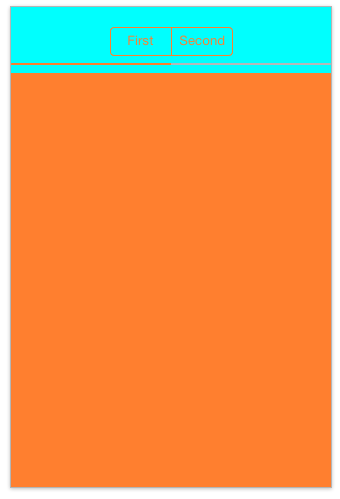
\includegraphics[width=\iphonewidth]{img/al_21.png}
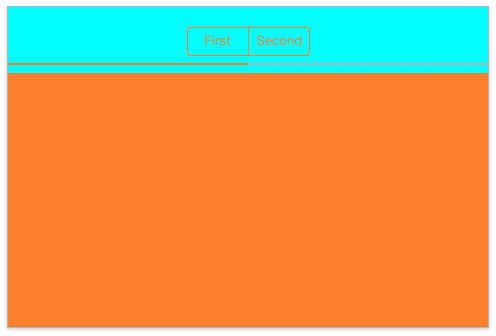
\includegraphics[height=\iphonewidth]{img/al_22.png}
\end{center}

\item Zwei Buttons im Abstand von 20pt sind am oberen Bildschirmrand zusammen horizontal zentriert. Ein \objc{UISlider} mit zugehörigem Label und eine füllende View befinden sich darunter. Ändern wir den Text der Label, passt sich das Layout an.
\begin{center}
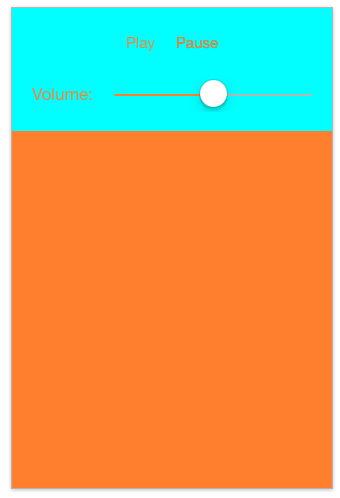
\includegraphics[width=\iphonewidth]{img/al_31.png}
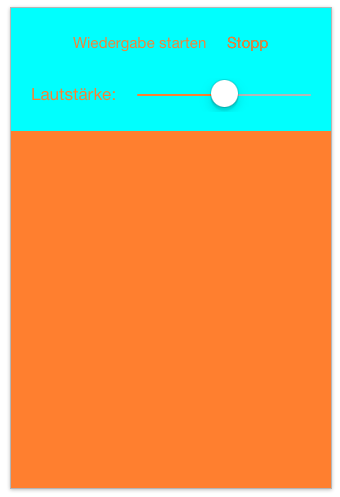
\includegraphics[width=\iphonewidth]{img/al_32.png}
\end{center}

\item Zwei Views haben (Platzhalter-) Intrinsic Content Sizes von 300x300pt und 100x100pt. Die größere wird wenn möglich vertikal zentriert, hat jedoch immer einen Abstand von mindestens 20pt zur darunter befindlichen kleineren View. Beide sind horizontal zentriert. Die kleinere View ist außerdem immer mindestens 20pt vom unteren Bildschirmrand entfernt. Wird der verfügbare Platz kleiner, wird die größere View vor der kleineren gestaucht.
\begin{center}
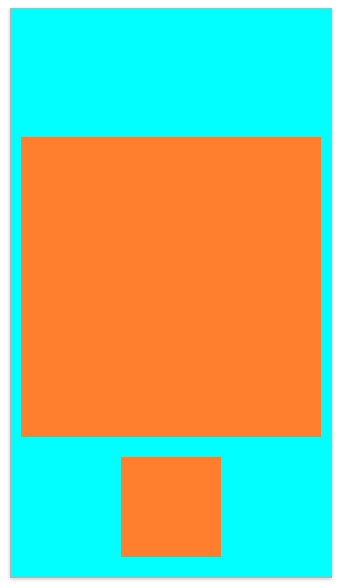
\includegraphics[width=\iphonewidth]{img/al_11.png}
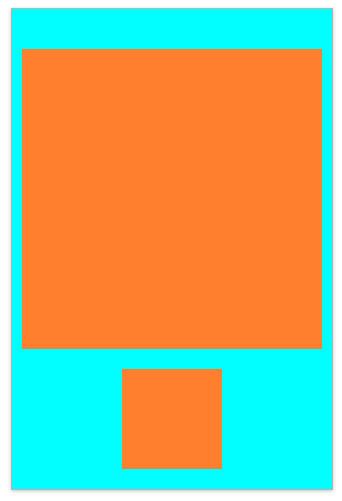
\includegraphics[width=\iphonewidth]{img/al_12.png}
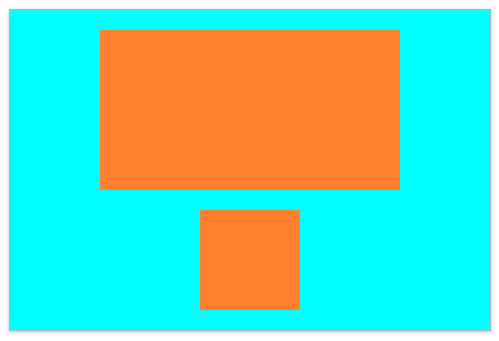
\includegraphics[height=\iphonewidth]{img/al_13.png}
\end{center}

\item Drei Views füllen jeweils den verfügbaren vertikalen Platz mit einem Abstand von 20pt zur Begrenzung. Horizontal sind sie gleichmäßig verteilt.
\begin{center}
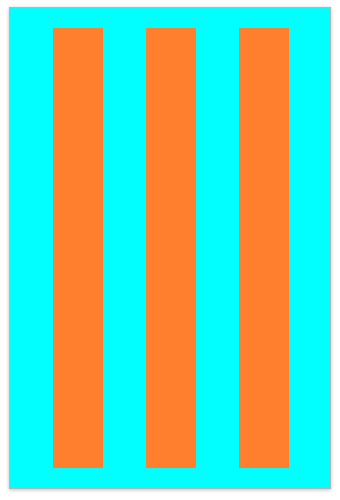
\includegraphics[width=\iphonewidth]{img/al_02.png}
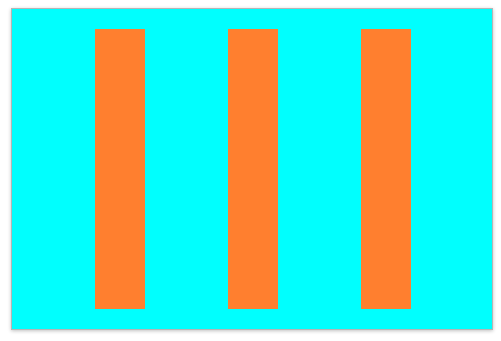
\includegraphics[height=\iphonewidth]{img/al_01.png}
\end{center}

\end{enumerate}

\exchinweis{In einigen Situationen kann die Verwendung von unsichtbaren Views als Platzhalter hilfreich sein. Dafür kann das Attribut \objc{BOOL hidden} verwendet werden, das auch im Storyboard verfügbar ist.}

\end{excitem}

\end{exc}


\chapter{Cities}

iOS Apps bestehen im Allgemeinen nicht nur aus einer, sondern aus einer Vielzahl von untereinander verbundenen Bildschirmansichten. Wir haben gelernt, dass jede Komponente der Benutzeroberfläche letztendlich von einem \objc{UIView} Objekt in der View Hierarchie des übergeordneten \objc{UIWindow} Objekts dargestellt wird.

Nun können wir die View Hierarchie einer komplexen App natürlich nicht wie im vorherigen Abschnitt zentral im App Delegate verwalten \excref{exc:view_hierarchy}. Um eine sinnvolle Struktur zu schaffen, implementieren wir stattdessen \strong{View Controller}.

Diese sind der Controller-Komponente des Model-View-Controller Konzepts zugeordnet und im Skript ausführlich beschrieben.

Mit dieser App lernen wir das \strong{View Controller Containment} Prinzp kennen, schreiben eigene \objc{UIViewController} Subklassen und verwenden einige wichtige View Controller aus dem UIKit Framework.

\skriptref{View Controller Hierarchie}

\section{One City}

Wir wollen zunächst einen Buttons mit dem Titel einer Stadt implementieren und Informationen über die entsprechende Stadt in einem separaten View Controller anzeigen, wenn der Benutzer auf den Button drückt.

\begin{enumerate}

\item Beginnen wir mit einem neuen Xcode Projekt nach dem 'Single View' Template und mit dem Product Name 'cities'. Es wird damit automatisch eine Klasse \objc{AppDelegate} und ein Storyboard hinzugefügt. Zusätzlich befindet sich bereits eine Subklasse \objc{ViewController : UIViewController} in unserem Projekt.

\item Die Klasse \objc{ViewController} möchten wir zunächst in \objc{CitiesViewController} umbenennen. Dazu verwenden wir Xcode's \strong{Refactor} Funktion. Markiert den Namen der Klasse an einer beliebigen Stelle im Code und wählt mit einem Rechtsklick im Kontextmenü \menuc{Refactor > Rename...} \abbref{img:refactor}. Geben wir nun den Namen \objc{CitiesViewController} ein und bestätigen den Dialog, benennt Xcode das Symbol an allen Stellen im Code, in Storyboards und in Dateinamen um.

\includegraphicsc[8cm]{img/refactor.png}{img:refactor}{Die Refactor Funktion ist sinnvoll, um Symbole im gesamten Projekt umzubennen}

\item Im Storyboard finden wir eine Scene mit einem Objekt dieser (nun umbenannten) \objc{CitiesViewController} Klasse. Wie im Skript dargestellt, können wir uns im Identity Inspector davon überzeugen, dass die Klasse des View Controller Objekts tatsächlich \objc{CitiesViewController} ist. Zur Laufzeit wird also ein solches Objekt erzeugt und dem \objc{UIWindow} Objekt als Root View Controller zugeordnet, da die Scene als 'Initial Scene' gekennzeichnet ist. Damit wird die Content View dieses View Controllers zu Beginn der Ausführung der App der View Hierarchie des \objc{UIWindow} Objekts hinzugefügt.

\item Ziehen wir nun \objc{UIView} Objekte auf die Content View des View Controllers, werden diese zur View Hierarchie der Content View hinzugefügt. Der View Controller ist für die Verwaltung seiner Content View zuständig. Daher stellen wir Verbindungen in Form von IBOutlets und IBActions her, um Zugriff auf die Objekte zu erhalten und um auf Benutzereingaben reagieren zu können.

Wir benötigen zunächst nur ein \objc{UIButton} Objekt mit dem Namen einer beliebigen Stadt \abbref{img:one_city_ui}. Es gibt natürlich auch Städte in Mittelerde, Panem und auf Naboo.

\includegraphicsc[\iphonewidth]{img/one_city_ui.png}{img:one_city_ui}{Ein Button soll bei Betätigung Informationen über die entsprechende Stadt anzeigen}

\item Obwohl wir uns in dieser App hauptsächlich mit der Controller-Komponente beschäftigen, sollten wir eine einfache Datenstruktur implementieren, die zu unserer App passt. So können wir Daten einfacher verarbeiten und weitergeben. Erstellt eine neue Klasse \objc{City : NSObject} und definiert die Attribute \objc{NSString *name} und \objc{UIImage *image}.

\begin{objclst}
// City.h

@interface City : NSObject

@property (strong, nonatomic) NSString *name;
@property (strong, nonatomic) UIImage *image;

@end
\end{objclst}

\begin{objclst}
// City.m

#import "City.h"

@implementation City

@end
\end{objclst}

\item Um nun einen Bildschirm zu präsentieren, der die Informationen der ausgewählten Stadt anzeigt, implementieren wir eine weitere Subklasse von \objc{UIViewController}. Erstellt also eine neue Klasse \objc{CityDetailViewController : UIViewController}. Dieser Klasse übergeben wir das ausgewählte \objc{City} Objekt und überlassen ihr die Konfiguration ihrer Content View entsprechend den Attributen des Objekts. Definiert also ein Attribut \objc{City *city} im Header der \objc{CityDetailViewController} Klasse.

\begin{objclst}
// CityDetailViewController.h

@class City; // Forward Declaration (s. Skript)

@interface CityDetailViewController : UIViewController

@property (strong, nonatomic) City *city;

@end
\end{objclst}

\item Nun verwenden wir wieder das Storyboard, um die Benutzerführung zu konfigurieren. Zieht ein View Controller Objekt aus der Object Library auf das Storyboard und platziert es neben dem Cities View Controller. Wählt nun im Identity Inspector des hinzugefügten View Controllers das Eingabefeld 'Class' und gebt den Namen der neuen \objc{UIViewController} Subklasse \objc{CityDetailViewController} ein.

\item Platziert ein \objc{UILabel} und ein \objc{UIImageView} Objekt in der Content View des \objc{CityDetailViewController} und verbindet sie mit IBOutlets im Code \abbref{img:city_detail_ui}. Fügt außerdem einen 'Zurück' Button hinzu und verbindet dessen \objc{UIControlEventTouchUpInside} Event mit einer IBAction. Diese können wir direkt implementieren:

\includegraphicsc[\iphonewidth]{img/city_detail_ui.png}{img:city_detail_ui}{Der City Detail View Controller soll Information über die ausgewählte Stadt anzeigen}

\begin{objclst}
// CityDetailViewController.m

#import "CityDetailViewController.h"

@interface CityDetailViewController ()

@property (strong, nonatomic) IBOutlet UILabel *nameLabel;
@property (strong, nonatomic) IBOutlet UIImageView *imageView;

- (IBAction)backButtonPressed:(id)sender;

@end

@implementation CityDetailViewController

- (IBAction)backButtonPressed:(id)sender {
    [self dismissViewControllerAnimated:YES completion:nil];
}

@end
\end{objclst}

Die Instanzmethode \objc{dismissViewControllerAnimated:completion:} von \objc{UIViewController} ist im Skript beschrieben.

\item Zur Präsentation des City Detail View Controllers können wir nun \strong{Segues} verwenden. Diese repräsentieren, wie im Skript beschrieben, Beziehungen zwischen einzelnen Scenes im Storyboard. Segues können analog zu IBOutlets und IBActions erstellt werden, indem eine Verbindungslinie mit gedrückter \keysc{\ctrlkey}-Taste gezogen wird. Wählt den Button im Cities View Controller aus und zieht eine Verbindung zum City Detail View Controller \abbref{img:one_city_detail_segue}. Erstellt so eine \strong{Modal Segue} zwischen Button und View Controller. Im Attributes Inspector könnt ihr die Segue konfigurieren und bspw. zwischen verschiedenen Übergangsanimationen auswählen.

\includegraphicsc{img/one_city_detail_segue.png}{img:one_city_detail_segue}{Eine Modal Segue konfiguriert die Präsentation des City Detail View Controllers bei Betätigung des Buttons}

\item Dem erstellten City Detail View Controller muss vor der Präsentation ein \objc{City} Objekt übergeben werden, damit er dessen Attribute darstellen kann. Dazu implementieren wir die Instanzmethode \objc{prepareForSegue:sender:} in unserer \objc{CitiesViewController} Klasse.

\begin{objclst}
// CitiesViewController.m

#import "CitiesViewController.h"
#import "City.h"
#import "CityDetailViewController.h"

@interface CitiesViewController ()

@end

@implementation CitiesViewController

- (void)prepareForSegue:(UIStoryboardSegue *)segue sender:(id)sender {
    City *city = [[City alloc] init];
    city.name = @"Melbourne";
    city.image = [UIImage imageNamed:@"melbourne"];
    CityDetailViewController *cityDetailVC = segue.destinationViewController;
    cityDetailVC.city = city;
}

@end
\end{objclst}

Hier erstellen wir bei dem Übergang zum City Detail View Controller ein neues \objc{City} Objekt und geben es an den City Detail View Controller weiter. Im Allgemeinen wird in einer solchen Situation natürlich auf die Model-Komponente der App zurückgegriffen.

Die Klassenmethode \objc{imageNamed:} von \objc{UIImage} lädt die Bilddatei mit dem angegebenen Dateinamen, sofern die Datei im Target referenziert ist. Für Dateien im PNG Format muss die Dateiendung nicht enthalten sein. Um dem Target eine Bilddatei hinzuzufügen, könnt ihr sie einfach auf die Dateiliste des Project Navigators ziehen. Später werden wir Xcode Asset Catalogs für die Bilddateien unserer Apps verwenden.

\item Schließlich müssen wir den City Detail View Controller für die Darstellung der Attribute des \objc{City} Objekts konfigurieren. Dies geschieht am besten in einer Implementierung der \objc{viewWillAppear:} Instanzmethode in der \objc{CityDetailViewController} Klasse.

\begin{objclst}
#import "CityDetailViewController.h"
#import "City.h"

@interface CityDetailViewController ()

@property (strong, nonatomic) IBOutlet UILabel *nameLabel;
@property (strong, nonatomic) IBOutlet UIImageView *imageView;

- (IBAction)backButtonPressed:(id)sender;

@end

@implementation CityDetailViewController

- (void)viewWillAppear:(BOOL)animated {
    [super viewWillAppear:animated];
    self.nameLabel.text = self.city.name;
    self.imageView.image = self.city.image;
}

- (IBAction)backButtonPressed:(id)sender {
    [self dismissViewControllerAnimated:YES completion:nil];
}

@end
\end{objclst}

\item Betätigt ihr nun den Button, wird die Content View des City Detail View Controller angezeigt und mit dem entsprechenden \objc{City} Objekt konfiguriert \abbref{img:one_city_run}.

\includegraphicsc[\iphonewidth]{img/one_city_run.png}{img:one_city_run}{Wird der Button betätigt, zeigt der City Detail View Controller die Informationen zu der ausgewählten Stadt}

\end{enumerate}

\begin{exc}
\begin{excitem}{cities}{Cities}

Implementiert diesen ersten Teil der Cities App, indem ihr die Schritte oben nachvollzieht.

\end{excitem}
\end{exc}


\section{One City Navigation}

UIKit stellt für diese häufig verwendete Master-Detail View Controller Hierarchie die Subklasse \objc{UINavigationController : UIViewController} zur Verfügung. Diese wird im Skript erläutert und eignet sich an dieser Stelle besser als Modal Segues.

\begin{enumerate}

\item Zieht einfach ein \objc{UINavigationController} Objekt aus der Object Library auf euer Storyboard. Dabei wird zusätzlich zu der Navigation Controller Scene automatisch eine weitere View Controller Scene als Root View Controller des Navigation Controllers hinzugefügt. Löscht diesen zusätzlichen View Controller und wählt stattdessen den \objc{CitiesViewController} als Root View Controller. Erstellt dafür eine \strong{Relationship Segue} zwischen beiden Objekten, indem ihr wieder mit gedrückter \keysc{\ctrlkey}-Taste eine Verbindung zieht. Markiert außerdem den Navigation Controller als Initial View Controller \abbref{img:nav_controller_segue}.

\includegraphicsc{img/nav_controller_segue.png}{img:nav_controller_segue}{Eine Relationship Segue markiert den Root View Controller eines Navigation Controllers}

\item Ihr könnt nun die Modal Segue zwischen \objc{CitiesViewController} und \objc{CityDetailViewController} auswählen und im Attributes Inspector den Typ zu \strong{Push Segue} ändern. Nun wird automatisch statt der \objc{presentViewController:animated:completion} Methode von \objc{UIViewController} die \objc{pushViewController:animated:} Methode von \objc{UINavigationController} aufgerufen, wenn die Segue ausgelöst wird.

\item Den 'Zurück' Button könnt ihr nun entfernen, da \objc{UINavigationController} einen eigenen Mechanismus implementiert und eine \objc{UINavigationBar} am oberen Bildschirmrand anzeigt. Auch die Labels werden nicht mehr benötigt. Stattdessen können wir das \objc{NSString *title} Attribut von \objc{UIViewController} verwenden, dessen Wert als Titel in der Navigation Bar angezeigt wird \abbref{img:nav_controller_ui}.

\includegraphicsc{img/nav_controller_ui.png}{img:nav_controller_ui}{Navigation Controller zeigen eine Navigation Bar an}

\begin{objclst}
// CityDetailViewController.m

#import "CityDetailViewController.h"
#import "City.h"

@interface CityDetailViewController ()

@property (strong, nonatomic) IBOutlet UIImageView *imageView;

@end

@implementation CityDetailViewController

- (void)viewWillAppear:(BOOL)animated {
    [super viewWillAppear:animated];
    ^\objchighlight{self.title = self.city.name;}^
    self.imageView.image = self.city.image;
}

@end
\end{objclst}

Verwendet außerdem gerne Auto Layout, um die Views zu positionieren.

\item Durch die Verwendung des Navigation Controllers erhält unsere App nun die Standardanimationen und -mechanismen aus UIKit, diese sich durch die Verwendung von Subklassen und sog. Delegates vielseitig anpassen lassen \abbref{img:nav_controller_run}.

\includegraphicsc[\iphonewidth]{img/nav_controller_run.png}{img:nav_controller_run}{Navigation Controller stellen Standardanimationen und -mechanismen zur Verfügung}

\end{enumerate}

\begin{exc}

\begin{excitem}{continents}{Continents}

Erweitert die App um einen View Controller, der die Städte in Kontinente (oder Planeten) einteilt. \strong{Alternativ könnt ihr natürlich auch gene kreativ werden und eine eigene App schreiben, in der zwischen verschiedenen View Controllern gewechselt wird!}

\begin{enumerate}
\item Wenn wir weitere Städte hinzufügen, kann es sinnvoll sein, sie in Kontinente (oder Planeten) einzuteilen. Erstellt eine neue Klasse \objc{Continent} und definiert analog zur \objc{City} Klasse die Attribute \objc{NSString *name} und \objc{UIImage *image}. Aufgrund der Analogien zwischen den beiden Klassen könnt ihr auch stattdessen eine Superklasse \objc{Location} erstellen, die die beiden Attribute definiert, und von der \objc{Continent} und \objc{City} abstammen.
\item Modifiziert die Benutzerführung der Cities App durch die Einführung eines neuen View Controllers \objc{ContinentsViewController}, der bei der Ausführung zuerst angezeigt werden soll. Konfiguriert einen Button mit dem Namen eines Kontinenten und stellt eine Push Segue Verbindung zum Cities View Controller her.
\item Implementiert die \objc{prepareForSegue:sender:} Methode des \objc{ContinentsViewController}. Übergebt hier einem neuen Attribut \objc{Continent *continent} des Cities View Controller ein \objc{Continent} Objekt entsprechend des betätigten Buttons.
\item Verwendet die \objc{viewWillAppear:} Methode, um den Kontinentnamen als Titel des Cities View Controller entsprechend des übergebenen \objc{Continent} Objekts anzuzeigen.
\item \excextra{Erweitert die Klasse \objc{Location} (bzw. \objc{Continent}) um ein Attribut \objc{NSArray *subLocations} für die enthaltenen Orte. Fügt den View Controllern \objc{ContinentsViewController} und \objc{CitiesViewController} jeweils einen weiteren Button für einen zweiten Ort hinzu. Versucht nun die Implementierungen anzupassen, sodass die Betätigung eines Buttons den entsprechenden Ort an den nächsten View Controller weitergibt. Die Cities View Controller soll also bswp. die Namen der beiden Städte an Position 0 und 1 des \objc{subLocations} Attributs des \objc{Continent} Objekts anzeigen. Eine Limitierung auf 2 Orte ist hier ausreichend, im nächsten Abschnitt werden wir für Situationen dieser Art dynamische Table Views verwenden.}
\end{enumerate}

\end{excitem}

\end{exc}


\section{More Cities}

Wenn wir eine Liste von Objekten darstellen wollen, konfigurieren wir natürlich nicht explizit Views für jedes Objekt. Stattdessen verwenden wir Subklassen von \objc{UITableViewController : UIViewController} und ihre Content Views der Klasse \objc{UITableView : UIView}, die mit dem \strong{Delegate Konzept} vielseitig einsetzbar sind.

\skriptref{Das Delegate Konzept, Table Views \& Table View Controller}

\begin{enumerate}

\item Wir möchten nun eine Liste von Städten anstatt einzelner Buttons anzeigen. Dafür ändern wir die Superklasse unseres \objc{CitiesViewController} von \objc{UIViewController} zu \objc{UITableViewController}. Außerdem können wir die IBOutlets entfernen.

\item Ein Table View Controller hat ein Objekt der \objc{UITableView} Klasse als Content View. Im Storyboard müssen wir daher die bisherige Content View mit einem Table View Objekt aus der Object Library ersetzen. Die Content View wird ersetzt, wenn wir die neue View einfach auf das View Controller Objekt im Navigationsbereich ziehen.

\strong{Hinweis:} Anstatt einen existierenden View Controller wie beschrieben in einen Table View Controller umzukonfigurieren, kann auch ein Table View Controller aus der Object Library gezogen werden.

\item Eine Table View kann, wie im Skript beschrieben, dynamischen oder statischen Inhalt darstellen. Im Attributes Inspector können wir den Modus 'Dynamic Properties' auswählen. Damit die Table View nun Inhalt präsentieren kann, benötigt sie \strong{Prototype Cells}, die den 'Bauplan' für jede Zelle dieser Art definieren. Fügt dafür eine \objc{UITableViewCell} aus der Object Library hinzu oder erhöht die entsprechende Zahl im Attributes Inspector um 1.

\item Wir können Prototype Cells nun entweder nach Belieben mit Subviews konfigurieren, oder im Attributes Inspector einen Standardstil auswählen. Wählt hier zunächst 'Basic' \abbref{img:morecities_prototypecells}.

\includegraphicsc[\iphonewidth]{img/morecities_prototypecells.png}{img:morecities_prototypecells}{Prototype Cells dienen als Vorlage für die Zellen der Table View}

\item Um Prototype Cells zu identifizieren, sollte ihnen ein \strong{Reuse Identifier} im Attributes Inspector zugeordnet werden. Tippt hier 'cityCell' ein.

\item Da unsere Table View dynamischen Inhalt anzeigen soll, können wir diesen nicht im Storyboard konfigurieren. Stattdessen verwendet die Table View das \strong{Delegate Kozept}, um Daten zu 'erfragen', wenn sie sie benötigt. Dazu ruft das \objc{UITableView} Objekt Methoden auf einem Delegate Objekt auf, die in einem \strong{Protokoll} definiert sind. \objc{UITableView} teilt diese Anfragen in die \objc{UITableViewDatasource} und \objc{UITableViewDelegate} Protokolle auf. Um den entsprechenden Attributen \objc{id<UITableViewDatasource> datasource} und \objc{id<UITableViewDelegate> delegate} Objekte zuzuweisen, sind diese als IBOutlets markiert. Zieht also zwei Verbindungen von der Table View zum \objc{CitiesViewController} und wählt diesen damit sowohl als Delegate als auch als Datasource.

\item Im Allgemeinen repräsentiert eine Table View ein \objc{NSArray}. Definiert also im Interface des \objc{CitiesViewController} ein Attribut \objc{NSArray *cities} und überschreibt die Getter Methode des Attributs, um die Liste auf Anfrage zu erstellen und zurückzugeben:

\begin{objclst}
#import "CitiesViewController.h"
#import "City.h"

@interface CitiesViewController ()

@property (strong, nonatomic) NSArray *cities;

@end

@implementation CitiesViewController

- (NSArray *)cities {
    /* Da wir die Getter Methode hier überschreiben, können wir nicht self.cities verwenden, da die Dot-Syntax die Getter Methode aufruft (Endlosschleife). Stattdessen verwenden wir die ebenfalls (für jede Property) automatisch generierte Instanzvariable _cities (s. Skript). */
    if (!_cities) {

        City *melbourne = [[City alloc] init];
        melbourne.name = @"Melbourne";
        melbourne.image = [UIImage imageNamed:@"melbourne"];
        City *sydney = [[City alloc] init];
        sydney.name = @"Sydney";
        sydney.image = [UIImage imageNamed:@"sydney"];
        City *brisbane = [[City alloc] init];
        brisbane.name = @"Brisbane";
        brisbane.image = [UIImage imageNamed:@"brisbane"];
        City *adelaide = [[City alloc] init];
        adelaide.name = @"Adelaide";
        adelaide.image = [UIImage imageNamed:@"adelaide"];
        City *perth = [[City alloc] init];
        perth.name = @"Perth";
        perth.image = [UIImage imageNamed:@"perth"];
        City *canberra = [[City alloc] init];
        canberra.name = @"Canberra";
        canberra.image = [UIImage imageNamed:@"canberra"];

        _cities = @[melbourne, sydney, brisbane, adelaide, perth, canberra];
    }
    return _cities;
}

@end
\end{objclst}

\item Als Subklasse von \objc{UITableViewController} erbt \objc{CitiesViewController} leere Implementierungen der \objc{UITableViewDatasource} und \objc{UITableViewDelegate} Protokolle. Wir können diese nun überschreiben, um unsere Tabelle mit Daten zu füllen. Dabei sind zunächst die drei erforderlichen Methoden zur Darstellung einer dynamischen Table View zu implementieren:

\begin{objclst}
#pragma mark - Table View Datasource

- (NSInteger)numberOfSectionsInTableView:(UITableView *)tableView {
    return 1;
}

- (NSInteger)tableView:(UITableView *)tableView numberOfRowsInSection:(NSInteger)section {
    return [self.cities count];
}

- (UITableViewCell *)tableView:(UITableView *)tableView cellForRowAtIndexPath:(NSIndexPath *)indexPath {

    // Greift auf das Model zurück, um das darzustellende Objekt zu erhalten
    City *city = [self.cities objectAtIndex:indexPath.row];

    // Erstellt ein neues UITableViewCell Objekt entsprechend der im Storyboard definierten Prototype Cell mit dem gegebenen Identifier oder verwendet eine existierende, momentan nicht verwendete Zelle mit diesem Identifier
    UITableViewCell *cell = [tableView dequeueReusableCellWithIdentifier:@"cityCell"];

    // Konfiguriert die View entsprechend des Models
    cell.textLabel.text = city.name;
    cell.imageView.image = city.image;

    return cell;
}
\end{objclst}

\objc{#pragma mark} kennzeichnet eine Überschrift ähnlich eines Kommentars und wird zusätzlich in der Jump Bar angezeigt. Ein Bindestrich \objc{-} erzeugt dort eine horizontale Trennlinie

\item Diese drei Methoden des \objc{UITableViewDatasource} Protokolls stellen der Table View die erforderlichen Informationen zur Verfügung, um die Tabelle anzeigen zu können \abbref{img:cities_tableview}.

\includegraphicsc[\iphonewidth]{img/cities_tableview.png}{img:cities_tableview}{Eine Table View stellt Anfragen an ihr Datasource und Delegate Objekt, um Zellen dynamisch anzuzeigen}

\item Die Präsentation des Detail City View Controllers kann nun erneut mithilfe von Segues realisiert werden. Dazu können wir im Storyboard eine Push Segue von der Prototype Cell zum Detail City View Controller erstellen.

\item Da diese Segue nun von jeder Zelle ausgelöst wird, die nach Vorlage der Prototype Cell erstellt wurde, müssen wir in der \objc{prepareForSegue:sender:} Methode zunächst den Index Path der betätigten Zelle herausfinden. Damit lässt sich anschließend das entsprechende Model Objekt erhalten und der City Detail View Controller konfigurieren.

\begin{objclst}
- (void)prepareForSegue:(UIStoryboardSegue *)segue sender:(id)sender {

    NSIndexPath *indexPath = [self.tableView indexPathForCell:sender];
    City *city = [self.cities objectAtIndex:indexPath.row];

    CityDetailViewController *cityDetailVC = segue.destinationViewController;
    cityDetailVC.city = city;
}
\end{objclst}

\end{enumerate}

\begin{exc}

\begin{excitem}{tableviews}{Table Views}

Verwendet nun analog auch für den Continents View Controller aus der vorherigen Übungsaufgabe eine dynamische Table View \strong{oder schreibt eine andere App, die Table Views verwendet}.

Ersetzt dazu die Content View des Continents View Controllers im Storyboard mit einer Table View, ändert dessen Klasse zu \objc{UITableViewController} und implementiert die benötigten Methoden der \objc{UITableViewDatasource} und objc{UITableViewDelegate} Protokolle.

\exchinweis{Vergesst nicht, der Table View den Continents View Controller als Datasource und Delegate Objekt zuzuweisen, sodass die Methoden überhaupt aufgerufen werden. Im Storyboard stehen dazu die IBOutlets der Table View zur Verfügung.}

\end{excitem}

\end{exc}


\chapter{Seasonizer}

Mit den Apps der vergangenen Vorlesungen haben wir die Grundlagen der Programmierung für iOS Geräte und einige wichtige Architekturkonzepte kennengelernt. Mit diesem Wissen lässt sich bereits ein Großteil der zur Verfügung stehenden Frameworks anwenden und viele Funktionen, die iOS Geräte bieten, in unsere eigenen Apps integrieren.

Aus gegebenem Anlass implementieren wir in dieser App einige häufig verwendete Funktionen wie Multi-Touch Gesten und Kamera Integration, um beim nächsten Familienfest nicht nur mit unseren neu erworbenen Programmierfähigkeiten anzugeben, sondern auch noch Fotos von Familienmitgliedern festlich dekorieren zu können \abbref{img:seasonizer}.

\includegraphicsc[\iphonewidth]{img/seasonizer.png}{img:seasonizer}{Mit der Seasonizer App lassen sich Familienmitglieder festlich dekorieren und ungewollte Haarfarben verdecken}

\subsubsection{Funktionen der Seasonizer App}

\emph{Das Schneeflockensystem kennzeichnet die Schwierigkeit der Funktion von * (machbar) bis *** (unmöglich).}

\begin{description}
\item [*] Die App besitzt eine Hauptansicht mit Navigation Bar und Toolbar. Den Inhalt füllt eine Image View für das Foto und eine darüberliegende View mit transparentem Hintergrund für die Accessories.
\item [*] Es gibt einen Button in der Toolbar, mit dem ein Foto von der Kamera oder Foto Bibliothek ausgewählt werden kann, das anschließend von der Image View angezeigt wird.
\item [**] Ein weiterer Button zeigt modal eine Liste von Accessories an. Wird ein Accessory ausgewählt, wird es der Hauptansicht hinzugefügt.
\item [**] Die Accessories lassen sich mit Gesten verschieben, skalieren, drehen und löschen.
\item [*] Mit einem Action Button kann das Bild über verschiedene Kanäle wie Nachrichten, Email oder Facebook verteilt werden.
\item [**] Die Elemente wie Bild und Accessories werden gespeichert und beim nächsten Start der App wiederhergestellt.
\item [*] Ein Toolbar Button dient dem Zurücksetzen der Benutzeroberfläche.
\item [extra] Es schneit in der App!
\item [extra] Implementiert, was euch einfällt! Ich bin auf eure Ideen gespannt.
\end{description}

Anders als für die bisherigen Apps wird es an dieser Stelle keine vollständige Schritt-für-Schritt Anleitung geben. Versucht stattdessen, die Funktionen der App zu implementieren, indem ihr die Hinweise und die Informationen der bisherigen Themen anwendet. Ich stehe dabei natürlich jederzeit gerne für Fragen zur Verfügung.

\subsubsection{Hinweise}

\begin{itemize}

\item Wenn ihr mit dem \emph{Single View} Template beginnt, bietet es sich an, dem View Controller der Hauptansicht einen sinnvollen Namen wie \objc{CanvasViewController} zu geben. Verwendet außerdem den Project Name \emph{seasonizer}.

\item \strong{Navigation Bar und Toolbar} lassen sich sehr einfach anzeigen, wenn ein Navigation Controller verwendet wird. Buttons lassen sich dann als Objekte der \objc{UIBarButtonItem} Klasse aus der Object Library dem Navigation Item hinzufügen. \objc{UIBarButtonItem} bietet bereits viele Stile wie \objc{UIBarButtonSystemItemCamera} zur Auswahl im Attributes Inspector an.

\item Die Auswahl zwischen \strong{Kamera und Foto Bibliothek} lässt sich sinnvoll mit einem \objc{UIActionSheet} implementieren:

\begin{objclst}
- (IBAction)cameraButtonPressed:(id)sender {
    UIActionSheet *actionSheet = [[UIActionSheet alloc] initWithTitle:nil delegate:self cancelButtonTitle:@"Abbrechen" destructiveButtonTitle:nil otherButtonTitles:@"Kamera", @"Foto Bibliothek", nil];
    [actionSheet showFromToolbar:self.navigationController.toolbar];
}
\end{objclst}

Der View Controller muss nun als Empfänger des \objc{UIActionSheetDelegate} Protokolls markiert werden und die Delegate Methode \objc{actionSheet:clickedButtonAtIndex:} implementieren. Hier können wir einen \objc{UIImagePickerController} anzeigen, der als \objc{UIImagePickerControllerSourceTypeCamera} oder \objc{UIImagePickerControllerSourceTypePhotoLibrary} konfiguriert werden kann.

\begin{objclst}
- (void)actionSheet:(UIActionSheet *)actionSheet clickedButtonAtIndex:(NSInteger)buttonIndex {
    if (buttonIndex==actionSheet.cancelButtonIndex) return;
    
    // Der erste Button zeigt die Kamera, der zweite die Photo Library
    UIImagePickerControllerSourceType sourceType = (buttonIndex==actionSheet.firstOtherButtonIndex) ? UIImagePickerControllerSourceTypeCamera : UIImagePickerControllerSourceTypePhotoLibrary;
    
    // Für Geräte ohne Kamera muss die Verfügbarkeit des Source Types getestet werden
    if (![UIImagePickerController isSourceTypeAvailable:sourceType]) {
        UIAlertView *alertView = [[UIAlertView alloc] initWithTitle:@"Option nicht verfügbar" message:@"Dieses Gerät unterstützt diese Option nicht." delegate:nil cancelButtonTitle:@"Ok" otherButtonTitles:nil];
        [alertView show];
        return;
    }
    
    // Den UIImagePickerController erstellen, konfigurieren und anzeigen
    UIImagePickerController *imagePickerC = [[UIImagePickerController alloc] init];
    imagePickerC.delegate = self;
    imagePickerC.sourceType = sourceType;
    [self presentViewController:imagePickerC animated:YES completion:nil];
}
\end{objclst}

Der \objc{UIImagePickerController} verwendet abermals das Delegate Konzept, also muss der View Controller nun außerdem als Empfänger des \objc{UIImagePickerControllerDelegate} Protokolls markiert werden und folgende Methoden implementieren:

\begin{objclst}
- (void)imagePickerController:(UIImagePickerController *)picker didFinishPickingMediaWithInfo:(NSDictionary *)info {
    [picker dismissViewControllerAnimated:YES completion:nil];
    
    self.photoImageView.image = [info objectForKey:UIImagePickerControllerOriginalImage];
    
}
- (void)imagePickerControllerDidCancel:(UIImagePickerController *)picker {
    [picker dismissViewControllerAnimated:YES completion:nil];
}
\end{objclst}

\item Wir arbeiten in dieser App mit \strong{Accessory Objekten}, die jeweils ein Bild repräsentieren und Eigenschaften wie Titel haben können. Daher bietet es sich an, eine Klasse \objc{Accessory : UIImageView} zu erstellen. Objekten dieser Klasse erben dann die Darstellungsmechanismen der \objc{UIImageView} Klasse und es können Attribute wie \objc{NSString *title} hinzugefügt werden.

\item Um modal einen weiteren View Controller mit Titelleiste für die \strong{Accessory Liste} anzuzeigen, kann dieser wiederum in einem Navigation Controller verpackt werden \abbref{img:seasonizer_ui}. Es sollte eine dynamische Table View in einer Subklasse \objc{AccessoryListViewController : UITableViewController} verwendet werden, um die Liste der verfügbaren Accessories anzuzeigen.

\includegraphicsc{img/seasonizer_ui.png}{img:seasonizer_ui}{Navigation Controller bieten eine einfache Möglichkeit, Navigationsleisten und Toolbars anzuzeigen}

\item Der Accessory List View Controller kann ein privates Attribut \objc{NSArray *accessories} mit überschriebener Getter Methode implementieren, das der dynamischen Table View als Informationsquelle dient.

\begin{objclst}
- (NSArray *)accessories {
    if (!_accessories) {
        
        Accessory *antlers = [[Accessory alloc] init];
        antlers.title = @"Geweih";
        antlers.image = [UIImage imageNamed:@"reindeer_antlers"];

        Accessory *santaHat = [[Accessory alloc] init];
        santaHat.title = @"Weihnachtsmannmütze";
        santaHat.image = [UIImage imageNamed:@"santa_hat"];
        
        // ...
        
        _accessories = @[antlers, santaHat];
    }
    return _accessories;
}
\end{objclst}

\item Ihr könnt Bilddateien entweder direkt ins Projekt ziehen und so referenzieren, oder \strong{Asset Catalogs} verwenden. Im Projekt befindet sich bereits eine \emph{.xcassets} Datei, in der leere Referenzen zu App Icon und Launch Image zu finden sind. Hier könnt ihr einfach weitere Bilddateien auf den linken Listenbereich bewegen. Ein \strong{Image Set} besteht dabei immer aus einer Bilddatei mit normaler und einer mit doppelter Auflösung für Geräte mit Retina Display. Abhängig vom ausführenden Gerät wird hier immer die korrekte Datei geladen. Dies funktioniert ebenfalls für referenzierte Bilddateien außerhalb von Asset Catalogs, die wie \emph{image.png} und \emph{image@2x.png} benannt sind.

\item Die Auswahl eines Accessories kann mithilfe eines eigenen Delegate Protokolls implementiert werden. Dazu benötigt der Accessory List View Controller ein öffentliches Attribut \objc{id <AccessorySelectionDelegate> delegate} und sollte das Protokoll in seinem Header definieren:

\begin{objclst}
// AccessoryListViewController.h

@class Accessory; // Forward Declaration
@protocol AccessorySelectionDelegate; // Forward Declaration

@interface AccessoryListViewController : UITableViewController

@property (weak, nonatomic) id <AccessorySelectionDelegate> delegate;

@end

@protocol AccessorySelectionDelegate

- (void)accessoryListViewController:(AccessoryListViewController *)accessoryListVC didSelectAccessory:(Accessory *)accessory;

@end
\end{objclst}

Nun kann das Delegate Objekt über die Auswahl eines Accessories informiert werden:

\begin{objclst}
// in AccessoryListViewController.m

- (void)tableView:(UITableView *)tableView didSelectRowAtIndexPath:(NSIndexPath *)indexPath {
    Accessory *accessory = [self.accessories objectAtIndex:indexPath.row];

    [self.delegate accessoryListViewController:self didSelectAccessory:accessory];
    
}
\end{objclst}

Wenn der Canvas View Controller den Accessory View Controller präsentiert, muss er dem \objc{delegate} Attribut zugewiesen werden:

\begin{objclst}
// in CanvasViewController.m

- (void)prepareForSegue:(UIStoryboardSegue *)segue sender:(id)sender {
    if ([segue.identifier isEqualToString:@"showAccessoryList"]) {
        // Der Accessory List View Controller ist nicht das direkte Ziel der Segue, sondern dessen Navigation Controller. Daher müssen wir dessen Top View Controller verwenden, der nun der Accessory List View Controller ist.
        AccessoryListViewController *accessoryListVC = (AccessoryListViewController *)[segue.destinationViewController topViewController];
        accessoryListVC.delegate = self;
    }
}
\end{objclst}

Der Canvas View Controller muss nun außerdem als Empfänger des \objc{AccessorySelectionDelegate} Protokolls markiert werden und dieses implementieren:

\begin{objclst}
// in CanvasViewController.m

- (void)accessoryListViewController:(AccessoryListViewController *)accessoryListVC didSelectAccessory:(Accessory *)accessory {
    
    [self addAccessory:accessory]; // Diese Methode muss noch implementiert werden
    
    // Passe initiale Position und Größe an
    [accessory sizeToFit];
    accessory.center = [accessory.superview convertPoint:accessory.superview.center fromView:accessory.superview.superview];

    [accessoryListVC dismissViewControllerAnimated:YES completion:nil];
}
\end{objclst}

\item Der Canvas View Controller kann die angezeigten Accessories mit einem Attribut \objc{NSMutableArray *accessories} verwalten. Dafür sollte er zwei Methoden \objc{addAccessory:} und \objc{removeAccessory:} implementieren:

\begin{objclst}
- (void)addAccessory:(Accessory *)accessory {
    if (!self.accessories) self.accessories = [[NSMutableArray alloc] init];
    
    [self.accessories addObject:accessory]; // add accessory to list
    [self.accessoryView addSubview:accessory]; // display accessory on screen
    
}

- (void)removeAccessory:(Accessory *)accessory {
    [accessory removeFromSuperview];
    [self.accessories removeObject:accessory];
}
\end{objclst}

\item Für die Manipulation der Accessories mit Gesten können wir \strong{Gesture Recognizer} verwenden. UIKit implementiert einige hilfreiche Subklassen von \objc{UIGestureRecognizer}, die bestimmt Multi-Touch Events auf der ihr zugewiesenen View erkennen und ihr Delegate Objekt darüber informieren. Also können wir den Canvas View Controller als Empfänger des \objc{UIGestureRecognizerDelegate} Protokolls markieren, Gesture Recognizer in der \objc{addAccessory:} Methode hinzufügen und die Delegate Methoden zum Bewegen, Skalieren, Rotieren und Löschen der Accessories implementieren.

\begin{objclst}
- (void)addAccessory:(Accessory *)accessory {
    if (!self.accessories) self.accessories = [[NSMutableArray alloc] init];
    
    [self.accessories addObject:accessory];
    [self.accessoryView addSubview:accessory];

    accessory.userInteractionEnabled = YES; // UIImageView empfängt im Allgemeinen keine Touch Events, daher müssen wir dies hier aktivieren

    // Bewegen
    UIPanGestureRecognizer *panGR = [[UIPanGestureRecognizer alloc] initWithTarget:self action:@selector(pan:)];
    panGR.delegate = self;
    [accessory addGestureRecognizer:panGR];
    
    // Skalieren
    UIPinchGestureRecognizer *pinchGR = [[UIPinchGestureRecognizer alloc] initWithTarget:self action:@selector(pinch:)];
    pinchGR.delegate = self;
    [accessory addGestureRecognizer:pinchGR];

    // Drehen
    UIRotationGestureRecognizer *rotateGR = [[UIRotationGestureRecognizer alloc] initWithTarget:self action:@selector(rotate:)];
    rotateGR.delegate = self;
    [accessory addGestureRecognizer:rotateGR];

    // Löschen
    UILongPressGestureRecognizer *tapGR = [[UILongPressGestureRecognizer alloc] initWithTarget:self action:@selector(tap:)];
    tapGR.delegate = self;
    [accessory addGestureRecognizer:tapGR];
    
}

#pragma mark Gestures

- (BOOL)gestureRecognizer:(UIGestureRecognizer *)gestureRecognizer shouldRecognizeSimultaneouslyWithGestureRecognizer:(UIGestureRecognizer *)otherGestureRecognizer {
    // Gesture Recognizer unterbrechen die Erkennung einer Geste bei der Erkennung einer anderen, wenn hier NO zurückgegeben wird. 
    return YES;
}

- (void)pan:(UIPanGestureRecognizer *)sender {
    [sender.view.superview bringSubviewToFront:sender.view];
    
    CGPoint translation = [sender translationInView:sender.view.superview];
    sender.view.center = CGPointMake(sender.view.center.x+translation.x, sender.view.center.y+translation.y);

    [sender setTranslation:CGPointZero inView:sender.view.superview];
}

- (void)pinch:(UIPinchGestureRecognizer *)sender {
    [sender.view.superview bringSubviewToFront:sender.view];
    
    sender.view.transform = CGAffineTransformScale(sender.view.transform, sender.scale, sender.scale);
    
    [sender setScale:1.];
}

- (void)rotate:(UIRotationGestureRecognizer *)sender {
    [sender.view.superview bringSubviewToFront:sender.view];

    sender.view.transform = CGAffineTransformRotate(sender.view.transform, sender.rotation);
    
    [sender setRotation:0.];
}

- (void)tap:(UILongPressGestureRecognizer *)sender {
    if (sender.state!=UIGestureRecognizerStateBegan) return;
    
    [self becomeFirstResponder];
    UIMenuController *menuController = [UIMenuController sharedMenuController];
    [menuController setMenuItems:@[[[UIMenuItem alloc] initWithTitle:@"Entfernen" action:@selector(removeAccessoryButtonPressed:)]]];
    [menuController setTargetRect:CGRectMake(sender.view.center.x, sender.view.center.y, 0, 0) inView:sender.view.superview];
    [menuController setMenuVisible:YES animated:YES];

    tappedAccessory = (Accessory *)sender.view;
}
- (BOOL)canBecomeFirstResponder {
    return YES;
}

- (void)removeAccessoryButtonPressed:(id)sender {
    [self removeAccessory:tappedAccessory];
}
\end{objclst}

Hier sei angemerkt, dass wir aufgrund des Zusammenspiels verschiedener Gesture Recognizer jeweils Delta-Bewegungen verwenden und auf die View anwenden, indem der jeweilige Gesture Recognizer bei jedem Methodenaufruf zurückgesetzt wird.

Der \objc{UILongPressGestureRecognizer} zeigt einen speziellen \objc{UIMenuController} zur Darstellung eines \emph{Entfernen} Buttons. Damit dieser korrekt angezeigt wird, muss die \objc{canBecomeFirstResponder} Methode implementiert werden. Außerdem müssen wir eine Referenz auf das entsprechende \objc{Accessory} Objekt zwischenspeichern, um es in der Action Methode weiterverwenden zu können. Dazu kann dem Klasseninterface ein Attribut oder, wie hier gezeigt, eine Instanzvariable hinzugefügt werden:

\begin{objclst}
@interface CanvasViewController () < /* viele Protokolle */ > {
    
    Accessory *tappedAccessory; // Instanzvariable
    
}

// Attribut- und Methodendefinitionen ...

@end

\end{objclst}

\item Die Integration eines \strong{Activity Sheets} zum Teilen von Inhalten ist denkbar einfach. UIKit stellt dafür den \objc{UIActivityViewController} zur Verfügung, der eine Liste von Datenobjekten annimmt und abhängig vom Typ der Daten eine Auswahl von Kanälen zum Teilen anzeigt.

\begin{objclst}
- (IBAction)actionButtonPressed:(id)sender {
    UIActivityViewController *activityVC = [[UIActivityViewController alloc] initWithActivityItems:@[self.renderedPicture] applicationActivities:nil];
    [self presentViewController:activityVC animated:YES completion:nil];
}
\end{objclst}

In dieser Methode wird auf die Getter Methode eines Attributs \objc{UIImage *renderedPicture} zugegriffen. Dieses Attribut soll dazu dienen, auf das vollständige Bild zugreifen zu können. Es soll dieses aber nicht speichern, sondern bei jedem Aufruf neu generieren, da das Bild sich natürlich ändern kann. Also markieren wir das Attribut bei der Definition als \objc{readonly} und überschreiben dessen Getter Methode:

\begin{objclst}
// im Header
@property (readonly) UIImage *renderedPicture;
\end{objclst}

\begin{objclst}
// in der Implementierung
- (UIImage *)renderedPicture {
    UIGraphicsBeginImageContextWithOptions(self.canvasView.frame.size, YES, 0.);
    [self.canvasView drawViewHierarchyInRect:self.canvasView.bounds afterScreenUpdates:YES];
    UIImage *renderedPicture = UIGraphicsGetImageFromCurrentImageContext();
    UIGraphicsEndImageContext();
    return renderedPicture;
}
\end{objclst}

Hier wurde \objc{canvasView} im Storyboard als Superview der Image View (für das Foto) und der Accessory View (für die Accessories) konfiguriert.

\item Als kleines Extra können wir es in der App schneien lassen. Für graphische Spielereien dieser Art müssen wir etwas weiter in die Trickkiste greifen und mit dem \strong{Core Animation} Framework arbeiten. Fügt dem Projekt einfach eine Bilddatei \emph{snowflake.png} mit etwa 15x15 Pixelmaßen hinzu und verwendet folgenden Code:

\begin{objclst}
// in CanvasViewController.m

- (void)viewDidLoad {
    [super viewDidLoad];

    CAEmitterCell *cell = [CAEmitterCell emitterCell];
    cell.name = @"snowflake";
    cell.birthRate = 50.;
    cell.velocity = 30.;
    cell.velocityRange = cell.velocity;
    cell.yAcceleration = 10.;
    cell.spinRange = M_PI;
    cell.emissionLongitude = M_PI_2;
    cell.emissionRange = M_PI_4;
    cell.contents = (id)[UIImage imageNamed:@"snowflake"].CGImage;
    cell.lifetime = 7.;
    cell.alphaRange = 1.;
    cell.alphaSpeed = -1./cell.lifetime;
    
    CAEmitterLayer *emitter = [CAEmitterLayer layer];
    [emitter setEmitterCells:@[cell]];
    [emitter setFrame:self.navigationController.view.bounds];
    [emitter setEmitterPosition:CGPointMake(self.navigationController.view.bounds.size.width/2, -15.)];
    [emitter setEmitterSize:CGSizeMake(self.navigationController.view.frame.size.width, 0.)];
    [emitter setEmitterShape:kCAEmitterLayerRectangle];
    [emitter setRenderMode:kCAEmitterLayerAdditive];
    [self.navigationController.view.layer addSublayer:emitter];
    
}
\end{objclst}

\item Um die Benutzeroberfläche vollständig wiederherstellen zu können, müssen wir sowohl das Foto als auch die hinzugefügten Accessories speichern. Als Methode der Datenspeicherung bietet sich in dieser App die \strong{User Defaults} Mechanik an, doch auch das \strong{State Preservation} System könnte stattdessen verwendet werden.

Zur Speicherung der Accessories müssen wir in der \objc{Accessory : UIImageView} Klasse zunächst das \objc{NSCoding} Protokoll implementieren. Dieses Protokoll bietet die Möglichkeit, Objekte als \objc{NSData} zu serialisieren. \objc{UIImageView} implementiert dieses Protokoll bereits, daher müssen wir in der Subklasse lediglich die beiden Schlüsselmethoden überschreiben:

\begin{objclst}
- (void)encodeWithCoder:(NSCoder *)aCoder
{
    [super encodeWithCoder:aCoder];
    
    // encode properties
    [aCoder encodeObject:self.title forKey:@"title"];
}

- (id)initWithCoder:(NSCoder *)aDecoder
{
    if ((self = [super initWithCoder:aDecoder])) {
    
        // decode properties
        self.title = [aDecoder decodeObjectForKey:@"title"];
        
    }
    return self;
}
\end{objclst}

Nun können wir das \strong{Notifications} System verwenden, um über die Veränderung des App States informiert zu werden. Bewegt sich die App in den Hintergrund, sollen Bild und Accessories in den User Defaults gespeichert werden. In der \objc{viewDidLoad} Methode des Canvas View Controllers fügen wir diesen daher als Empfänger der \objc{UIApplicationDidEnterBackgroundNotification} hinzu und implementieren eine Methode, die bei Empfang einer solchen Notification aufgerufen wird:

\begin{objclst}
- (void)viewDidLoad
{
    [super viewDidLoad];
    
    [[NSNotificationCenter defaultCenter] addObserver:self selector:@selector(didEnterBackground:) name:UIApplicationDidEnterBackgroundNotification object:[UIApplication sharedApplication]];
    
    // ...
}

#define kUserDefaultsKeyPhotoImage @"image_data"
#define kUserDefaultsKeyAccessories @"accessory_data"

- (void)didEnterBackground:(NSNotification *)notification
{
    NSData *imageData = UIImagePNGRepresentation(self.photoImageView.image);
    [[NSUserDefaults standardUserDefaults] setObject:imageData forKey:kUserDefaultsKeyPhotoImage];

    NSData *accessoryData = [NSKeyedArchiver archivedDataWithRootObject:self.accessories]; // NSArray und alle enthaltenen Objekte der Klasse Accessory implementieren das NSCoding Protokoll und können somit archiviert werden
    [[NSUserDefaults standardUserDefaults] setObject:accessoryData forKey:kUserDefaultsKeyAccessories];
}
\end{objclst}

Die Wiederherstellung dieser gesicherten Daten kann nun in der \objc{viewDidLoad} Methode erfolgen:

\begin{objclst}
- (void)viewDidLoad
{
    [super viewDidLoad];
        
    NSData *imageData = [[NSUserDefaults standardUserDefaults] objectForKey:kUserDefaultsKeyPhotoImage];
    self.photoImageView.image = [UIImage imageWithData:imageData];
    
    NSData *accessoryData = [[NSUserDefaults standardUserDefaults] objectForKey:kUserDefaultsKeyAccessories];
    NSArray *accessories = [NSKeyedUnarchiver unarchiveObjectWithData:accessoryData];
    for (Accessory *accessory in accessories) {
        [self addAccessory:accessory];
    }
    
    // ...
}
\end{objclst}

Hier verwenden wir die \objc{addAccessory:} Methode, um die Accessories der View Hierarchie hinzuzufügen und die Gesture Recognizer zu erzeugen. In der vorherigen Version dieses Dokuments wurde in der \objc{addAccessory:} Methode außerdem die Position und Größe des neuen Accessories angepasst. Dies kann jedoch stattdessen in der Delegate Methode \objc{accessoryListViewController:didSelectAccessory:} geschehen. Beide Methoden sind oben in der veränderten Form zu finden.

\item Implementieren wir einen weiteren Toolbar Button, der die Benutzeroberfläche bei Betätigung \strong{zurücksetzt}, sollte zunächst eine Schaltfläche zur Bestätigung erscheinen.

Dazu eignet sich wieder ein \objc{UIActionSheet}. Dieses muss jedoch in der Implementierung der Delegate Methoden von dem Action Sheet zur Auswahl zwischen Kamera und Fotobibliothek unterschieden werden. Eine Möglichkeit besteht in der Definition eines privaten Attributs für jedes der beiden Action Sheets in der \objc{CanvasViewController} Klasse. Dann können wir die Action Methode des Reset Buttons wie folgt implementieren:

\begin{objclst}
- (IBAction)resetButtonPressed:(id)sender
{
    UIActionSheet *actionSheet = [[UIActionSheet alloc] initWithTitle:nil delegate:self cancelButtonTitle:@"Abbrechen" destructiveButtonTitle:@"Zurücksetzen" otherButtonTitles:nil];
    self.resetActionSheet = actionSheet; // dient der Identifikation des Action Sheets in der Delegate Methode
    [actionSheet showFromToolbar:self.navigationController.toolbar];
}
\end{objclst}

Analog muss die \objc{cameraButtonPressed:} Methode um die Attributzuweisung \objc{self.photoActionSheet = actionSheet} erweitert werden.

In der \objc{UIActionSheetDelegate} Methode \objc{actionSheet:clickedButtonAtIndex:} können wir nun eine Fallunterscheidung zwischen den Action Sheets durchführen:

\begin{objclst}
- (void)actionSheet:(UIActionSheet *)actionSheet clickedButtonAtIndex:(NSInteger)buttonIndex
{
    if (buttonIndex==actionSheet.cancelButtonIndex) return;
    
    if (actionSheet==self.resetActionSheet&&buttonIndex==actionSheet.destructiveButtonIndex)         {
        
        [self resetCanvas]; // muss noch implementiert werden
        
    } else if (actionSheet==self.photoActionSheet) {
        
        // ...
        
    }
}
\end{objclst}

In einer Methode \objc{resetCanvas} kann die Benutzeroberfläche dann zurückgesetzt werden:

\begin{objclst}
- (void)resetCanvas
{
    self.photoImageView.image = nil;
    
    [self.accessories makeObjectsPerformSelector:@selector(removeFromSuperview)];
    self.accessories = nil;
}
\end{objclst}

\end{itemize}


\chapter{Versionskontrolle mit Git}

Im Skript sind die Vorzüge der Versionskontrolle mit Git beschrieben. Anhand einer unserer Apps, bspw. der Seasonizer App, können wir die beschriebenen Grundlagen anwenden.

\skriptref{Versionskontrolle mit Git}

\begin{enumerate}

\item Da Git in erster Linie ein Kommandozeilenprogramm ist, verwenden wir zunächst die Terminal App. Später können wir auch bspw. die in Xcode integrierten Benutzeroberflächen verwenden. Öffnet die Terminal App und navigiert in den Ordner, der das Xcode Projekt beinhaltet. Dazu ist es hilfreich, zunächst \sh{cd} zu tippen und den Ordner dann auf das Terminal Fenster zu ziehen, wobei der Pfad automatisch eingegeben wird.

\begin{shlst}
cd path/to/project
\end{shlst}

\item Bei Erstellung des Projektes wurde möglicherweise bereits die Option ausgewählt, ein Git Repository zu initialisieren. Mit \sh{git status} können wir prüfen, ob hier bereits ein Git Repository existiert und es ansonsten mit \sh{git init} erstellen.

\begin{shlst}
git status
# Git Repository vorhanden:
>> # On branch master
>> nothing to commit, working directory clean
# kein Git Repository vorhanden:
>> fatal: Not a git repository (or any of the parent directories): .git
git init
\end{shlst}

\item Wir fügen dem Repository nun zunächst eine \sh{.gitignore} Datei hinzu, um verschiedene benutzerspezifische und temporäre Dateien des Xcode Projekts auszuschließen.

\begin{shlst}
touch .gitignore
open .gitignore
# Vorlage aus dem Skript kopieren
\end{shlst}

Nun können wir einen Commit ausführen, um die Datei dem Repository hinzuzufügen.

\begin{shlst}
git add .gitignore
git commit -m "Added .gitignore file"
\end{shlst}

Jederzeit kann es hilfreich sein, die Situation des Git Repositories mit \sh{git status} zu überprüfen. \sh{git log} zeigt außerdem die letzten Commits in der Konsole an.

\item Nun können wir an unserem Projekt weiterarbeiten und Änderungen an Dateien vornehmen. Verwendet bspw. die \objc{viewDidLoad} Methode des Initial View Controllers eurer App, um dessen Content View rot zu färben, oder ändert etwas anderes.

\begin{objclst}
- (void)viewDidLoad
{
    [super viewDidLoad];
    
    self.view.backgroundColor = [UIColor redColor];
}
\end{objclst}

In der Konsole sehen wir mit \sh{git status}, dass nun Änderungen vorliegen. Diese können wir in Form eines Commits im Git Repository speichern.

\begin{shlst}
git add filename # oder git add --all
git commit -m "Changed background color"
\end{shlst}

\item Es gibt viele verschiedene Möglichkeit der Commitnavigation und -manipulation. Wir können bspw. mit \sh{git checkout} einen bestimmten Commit laden, mit \sh{git reset} Commits entfernen oder sie mit \sh{git revert} in Form eines neuen Commits rückgängig machen. Dabei können wir einen bestimmten Commit anhand seines SHA hashs identifizieren, der bspw. mit \sh{git log} angezeigt wird, oder mit \sh{HEAD~x} den x-letzten Commit auswählen. Setzen wir den soeben ausgeführten Commit nun also bspw. zurück:

\begin{shlst}
git reset --hard HEAD~1
\end{shlst}

In der Dokumentation \linkref{http://git-scm.com/book/} kann sich ausführlich über die verschiedenen Möglichkeiten informiert werden.

\item Häufig wird Git zur Projektstrukturierung in Form von \strong{Feature Branches} eingesetzt. Nehmen wir also an wir unser Projekt liegt in seiner veröffentlichten Form vor. Möchten wir nun ein neues Feature implementieren oder Umstrukturierungen vornehmen, erstellen wir zunächst einen neuen Branch mit \sh{git branch}. Mit \sh{git checkout} wechseln wir das Arbeitsverzeichnis in diesen neuen Branch.

\begin{shlst}
git branch new_feature
git checkout new_feature
\end{shlst}

\item Nun können wir in diesem Branch an unserem Projekt arbeiten, ohne dass andere Branches verändert werden. Fügt bspw. wieder der \objc{viewDidLoad} Methode des Initial View Controllers einige Änderungen hinzu und führt einen Commit durch.

\begin{objclst}
- (void)viewDidLoad {
    [super viewDidLoad];
    
    UIAlertView *alert = [[UIAlertView alloc] initWithTitle:@"New Feature!" message:@"Is it a bug or a feature?" delegate:nil cancelButtonTitle:@"Bug" otherButtonTitles:@"Feature", nil];
    [alert show];
}
\end{objclst}

\begin{shlst}
git commit -a -m "Implemented new feature" # Der -a Flag fügt dem Commit automatisch veränderte Dateien hinzu
\end{shlst}

\item Erhalten wir nun plötzlich eine Email eines aufgebrachten Benutzers unserer App, der einen Bug gefunden hat, können wir problemlos zurück zum \sh{master} Branch wechseln und den Bug schnell beheben.

\begin{shlst}
git checkout master
# edit code to resolve bug
git commit -a -m "Resolved bug"
\end{shlst}

Nachdem wir zurück zum \sh{master} Branch gewechselt haben, sehen wir, dass die Änderungen des \sh{new_feature} Branches verschwunden sind. Stattdessen befindet sich der Code wieder in seinem ursprünglichen Zustand. Wir können den Bug also beheben, einen Commit ausführen und die App in der neuen Version veröffentlichen, um den Emailschreiber zu besänftigen.

Anschließend wechseln wir wieder in unseren Feature Branch und arbeiten dort weiter, wo wir unterbrochen wurden.

\begin{shlst}
git checkout new_feature
# more feature commits
\end{shlst}

\item Befindet sich der Feature Branch in einem Zustand, der veröffentlicht werden soll, muss er nur mit dem \sh{master} Branch vereinigt werden. Dazu führen wir einen Merge durch.

\begin{shlst}
git checkout master
git merge new_feature
\end{shlst}

Wurden im \sh{master} Branch keine weiteren Commits hinzugefügt, können die Commits des Feature Branches einfach angehängt werden (Fast-Forward). Gehen die Branches jedoch auseinander, versucht Git, die Änderungen zusammenzuführen. Mögliche Konflikte müssen dabei wie im Skript beschrieben im Code behoben werden.

Der Feature Branch kann anschließend gelöscht werden:

\begin{shlst}
git branch -d new_feature
\end{shlst}

\item Versionskontrolle ist nicht nur für größere Projekte essentiell und hilft bei der Entwicklung jeder iOS App, sondern ermöglicht auch die Zusammenarbeit mehrerer Entwickler an einem Projekt. Im Skript ist dieses Thema kurz beschrieben und auch auf den Service GitHub \linkref{http://www.github.com} verwiesen, der weltweit von Entwicklern verschiedenster Plattformen verwendet wird, um an Projekten zusammenzuarbeiten.

Auf GitHub ist bspw. meine Implementierung der Seasonizer App zu finden. Ihr könnt das Repository auf der Webseite einsehen \linkref{https://github.com/ios-dev-kurs/seasonizer} und herunterladen.

Navigiert dazu in der Konsole zu dem Verzeichnis eurer Projekte für diesen Kurs und führt \sh{git clone} aus.

\begin{shlst}
cd path/to/directory
git clone https://github.com/ios-dev-kurs/seasonizer
\end{shlst}

Das Repository wird dabei in das angegebene Verzeichnis heruntergeladen. Ihr könnt lokal daran weiterarbeiten und Commits durchführen. Wenn ich Änderungen am Remote Repository auf Github vornehme, können diese mit einem \sh{git pull} geladen und mit dem lokalen \sh{master} Branch zusammengeführt werden. Die lokalen Änderungen können jedoch nicht mit dem Remote Repository abgeglichen werden, da dazu die Zugangsdaten zu dem entsprechenden GitHub Account benötigt werden.

\item Github bietet für Situationen dieser Art das \strong{Fork} System an. Anstatt mein Repository direkt lokal zu Klonen, könnt ihr einen GitHub Account anlegen und den Fork Button \linkref{https://github.com/ios-dev-kurs/seasonizer/fork} meines Repositories klicken. Damit wird das Repository serverseitig auf eurem Account geklont. Ihr könnt es nun auf eurem Account finden und lokal klonen. Löscht dafür zunächst lokal das zuvor geklonte Repository.

\begin{shlst}
cd path/to/directory
git clone https://github.com/yourusername/seasonizer
\end{shlst}

Hier könnt ihr nun Commits durchführen und diese mit eurer serverseitigen Kopie meines Repositories abgleichen.

\begin{shlst}
# add commits ...
git push
\end{shlst}

Haltet ihr eure Änderungen für so genial oder notwendig, dass sie in mein Original Repository übernommen werden sollten, könnt ihr mir über die GitHub Webseite eine \strong{Pull Request} schicken, die mich auffordert, die einen Merge mit den Änderungen durchzuführen.

Andere Entwickler, die mein Repository geklont haben, können diese Änderungen anschließend herunterladen. In dieser Form kann ein Open Source Programmierprojekt weltweit von interessierten Entwicklern weiterentwickelt werden. Und dem Seasonizer sind damit keine Grenzen gesetzt.

\end{enumerate}

\end{document}
